% This document should be compiled with XeLaTeX. 
\documentclass[preprint,11pt,authoryear,3p]{elsarticle}

%% Use the option review to obtain double line spacing
%% \documentclass[preprint,review,12pt]{elsarticle}

%% Use the options 1p,twocolumn; 3p; 3p,twocolumn; 5p; or 5p,twocolumn
%% for a journal layout:
%% \documentclass[final,1p,times]{elsarticle}
%% \documentclass[final,1p,times,twocolumn]{elsarticle}
%% \documentclass[final,3p,times]{elsarticle}
%% \documentclass[final,3p,times,twocolumn]{elsarticle}
%% \documentclass[final,5p,times]{elsarticle}
%% \documentclass[final,5p,times,twocolumn]{elsarticle}

%% For including figures, graphicx.sty has been loaded in
%% elsarticle.cls. If you prefer to use the old commands
%% please give \usepackage{epsfig}
\usepackage{subfigure}

%% The amssymb package provides various useful mathematical symbols
\usepackage{amssymb}
%% The amsthm package provides extended theorem environments
% \usepackage{amsthm}
\usepackage{amsmath}

%% The lineno packages adds line numbers. Start line numbering with
%% \begin{linenumbers}, end it with \end{linenumbers}. Or switch it on
%% for the whole article with \linenumbers.
\usepackage{lineno}
\usepackage{lscape}
%% Set the font style of the main text as the times new roman
% \usepackage{fontspec}
% \setmainfont{Times New Roman}
% \renewcommand{\familydefault}{\rmdefault}

%% Add the command "\autoref{}"
\usepackage{hyperref}
%% Add the command "\hl{}"
\usepackage{soul, color, xcolor}
\usepackage{threeparttable}
\usepackage{longtable}
\usepackage{array}
\usepackage{setspace}

\biboptions{sort&compress}%参考文献可以压缩显示例如1-3

% \renewcommand{\figurename}{\bf{Fig.}} %修改标题样式
\renewcommand{\figureautorefname}{Fig.}
\renewcommand{\tablename}{\bf{Table}}
\renewcommand{\equationautorefname}{Eq.}
\renewcommand{\sectionautorefname}{Sec.}
\renewcommand{\subsectionautorefname}{Sec.}
\renewcommand{\subsubsectionautorefname}{Sec.}
\usepackage{caption}
\captionsetup[figure]{name={Fig.},labelsep=period}
\captionsetup[table]{name={Table},labelsep=period}
\captionsetup{labelfont=bf}

\usepackage{booktabs}
\usepackage{multirow}

%% Set the space between two lines of text next to each other.
\usepackage{setspace}
\renewcommand{\baselinestretch}{1.5}
% \setlength{\baselineskip}{24pt}


% \journal{Automation in Construction}

\begin{document}
% modify the line space between the text and equation.
\setlength{\abovedisplayskip}{-15pt}
% \setlength{\abovedisplayshortskip}{0pt}
\setlength{\belowdisplayskip}{-0pt}
% \setlength{\belowdisplayshortskip}{-12pt}

\begin{frontmatter}

%% Title, authors and addresses

%% use the tnoteref command within \title for footnotes;
%% use the tnotetext command for theassociated footnote;
%% use the fnref command within \author or \address for footnotes;
%% use the fntext command for theassociated footnote;
%% use the corref command within \author for corresponding author footnotes;
%% use the cortext command for theassociated footnote;
%% use the ead command for the email address,
%% and the form \ead[url] for the home page:
%% \title{Title\tnoteref{label1}}
%% \tnotetext[label1]{}
%% \author{Name\corref{cor1}\fnref{label2}}
%% \ead{email address}
%% \ead[url]{home page}
%% \fntext[label2]{}
%% \cortext[cor1]{}
%% \affiliation{organization={},
%%             addressline={},
%%             city={},
%%             postcode={},
%%             state={},
%%             country={}}
%% \fntext[label3]{}

\title{A State-of-the-Art Review on the Space-Air-Ground Integrated Intelligent Monitoring for Large-scale Deep Excavation Engineering}

%% use optional labels to link authors explicitly to addresses:
%% \author[label1,label2]{}
%% \affiliation[label1]{organization={},
%%             addressline={},
%%             city={},
%%             postcode={},
%%             state={},
%%             country={}}
%%
%% \affiliation[label2]{organization={},
%%             addressline={},
%%             city={},
%%             postcode={},
%%             state={},
%%             country={}}

% \author[Ori1,Ori2]{Qiwei Wan\fnref{firstAu}}
% \author[Ori1,Ori2]{Changjie Xu\corref{cor1}}
% \author[Ori3]{Xiangyu Wang}
% \author[Ori1,Ori2]{Haibin Ding}

% \fntext[firstAu]{School of Civil Engineering and Architecture, East China Jiaotong University, Nanchang 330021, China. \\ E-mail address: wqw@ecjtu.edu.cn}
% \cortext[cor1]{School of Civil Engineering and Architecture, East China Jiaotong University, Nanchang 330021,China. \\ E-mail address: xucj@zju.edu.cn}
% \address[Ori1]{State Key Laboratory of Safety and Resilience of Civil Engineering in Mountain Area, East China Jiaotong University,%Department and Organization
%             Nanchang,
%             330021,
%             Jiangxi,
%             China}

% \address[Ori2]{State Key Laboratory of Performance MonitoringProtecting of Rail Transit Infrastructure, East China Jiaotong University,%Department and Organization
%             Nanchang,
%             330021,
%             Jiangxi,
%             China}

% \address[Ori3]{Australasian Joint Research Centre for Building Information Modelling, Curtin University,%Department and Organization
%             GPO Box U1987,
%             Nanchang,
%             WA 6845,
%             Perth,
%             Australia}

\begin{abstract}

Space--Air--Ground (SAG) integrated monitoring is rapidly becoming the preferred strategy for safeguarding urban deep‐excavation projects. This study conducts a systematic review of 687 publications indexed in Web of Science and filters them to 522 high-quality papers using the Chinese Academy of Sciences (CAS) journal ranking. In parallel, six representative engineering case studies are analysed to trace the technical evolution and field performance of Interferometric Synthetic Aperture Radar (InSAR), Unmanned Aerial Vehicle (UAV) photogrammetry/Light Detection and Ranging (LiDAR), Global Navigation Satellite System (GNSS) positioning, and conventional ground instrumentation. Keyword co-occurrence analysis indicates a seven-fold rise in “InSAR” and a five-fold rise in “UAV” articles between 2010 and 2025, underscoring the boom in space- and air-borne technologies. A generic workflow that links data acquisition, heterogeneous data fusion, risk assessment, and decision support is proposed, together with eight mainstream fusion families—including Kalman filtering, Bayesian inference, Dempster-Shafer (D-S) evidence theory, and deep learning—each mapped to its excavation-specific strengths. Field evidence shows that dual- or tri-modal SAG configurations can keep wall-top displacement forecasts within ± 2 mm or $<$10 \% error while reducing life-cycle monitoring costs by an order of magnitude; for example, Persistent Scatterer Interferometry (PSI) replaced thousands of optical prisms during the post-excavation phase of London's Crossrail project. At Shanghai East Railway Station, a ground-only inclinometer array would cost more than USD 0.66 million, highlighting the cost-coverage advantage of space- and air-borne sensing. Nevertheless, persistent challenges remain: sensor-physics limits, data streams exceeding 5 GB day$^{-1}$, fragmented standards, and long-term reliability issues. Future research should prioritise physics-informed deep fusion, low-cost dense sensor networks, edge-cloud analytics, and high-revisit Synthetic Aperture Radar (SAR) constellations coupled with autonomous UAV swarms to deliver real-time, adaptive, and intelligent SAG monitoring.

\end{abstract}

%%Graphical abstract
% \begin{graphicalabstract}
% %\includegraphics{grabs}
% \end{graphicalabstract}

%%Research highlights
% \begin{highlights}
% \item Research highlight 1
% \item Research highlight 2
% \end{highlights}

\begin{keyword}
%% keywords here, in the form: keyword \sep keyword
% Multi-objective optimization \sep
% Enhanced genenic algorithm \sep
% Inverse design \sep
% Deformation control \sep
% Economic optimization 
%% PACS codes here, in the form: \PACS code \sep code

%% MSC codes here, in the form: \MSC code \sep code
%% or \MSC[2008] code \sep code (2000 is the default)

Space--Air--Ground monitoring \sep
Interferometric Synthetic Aperture Radar  \sep
Unmanned Aerial Vehicle photogrammetry \sep
Global Navigation Satellite System \sep
Multi-source data fusion \sep
Deep excavation
\end{keyword}

\end{frontmatter}

\linenumbers

\section{Introduction}

\subsection{Background and Challenges}

Large-scale deep excavation engineering, such as foundation pit excavation for urban infrastructure projects (e.g., subway tunnels, commercial buildings, and transport hubs), is a complex and high-risk activity \citep{gong2019advances}. A large-scale excavation project often involves multiple types of geotechnical engineering elements, such as slopes, roads, buildings, airports, etc., as shown in the \autoref{fig:complexEnvironment}. The stability and safety of these projects depend on real-time monitoring of ground deformation, displacement, and surrounding environmental conditions. Traditional monitoring methods, such as ground-based sensors (e.g., inclinometers, total stations), and optical remote sensing technologies, have been widely used in geotechnical engineering. However, these methods often face significant limitations in terms of spatial coverage, accuracy, and real-time performance. 

\begin{figure}
    \centering
    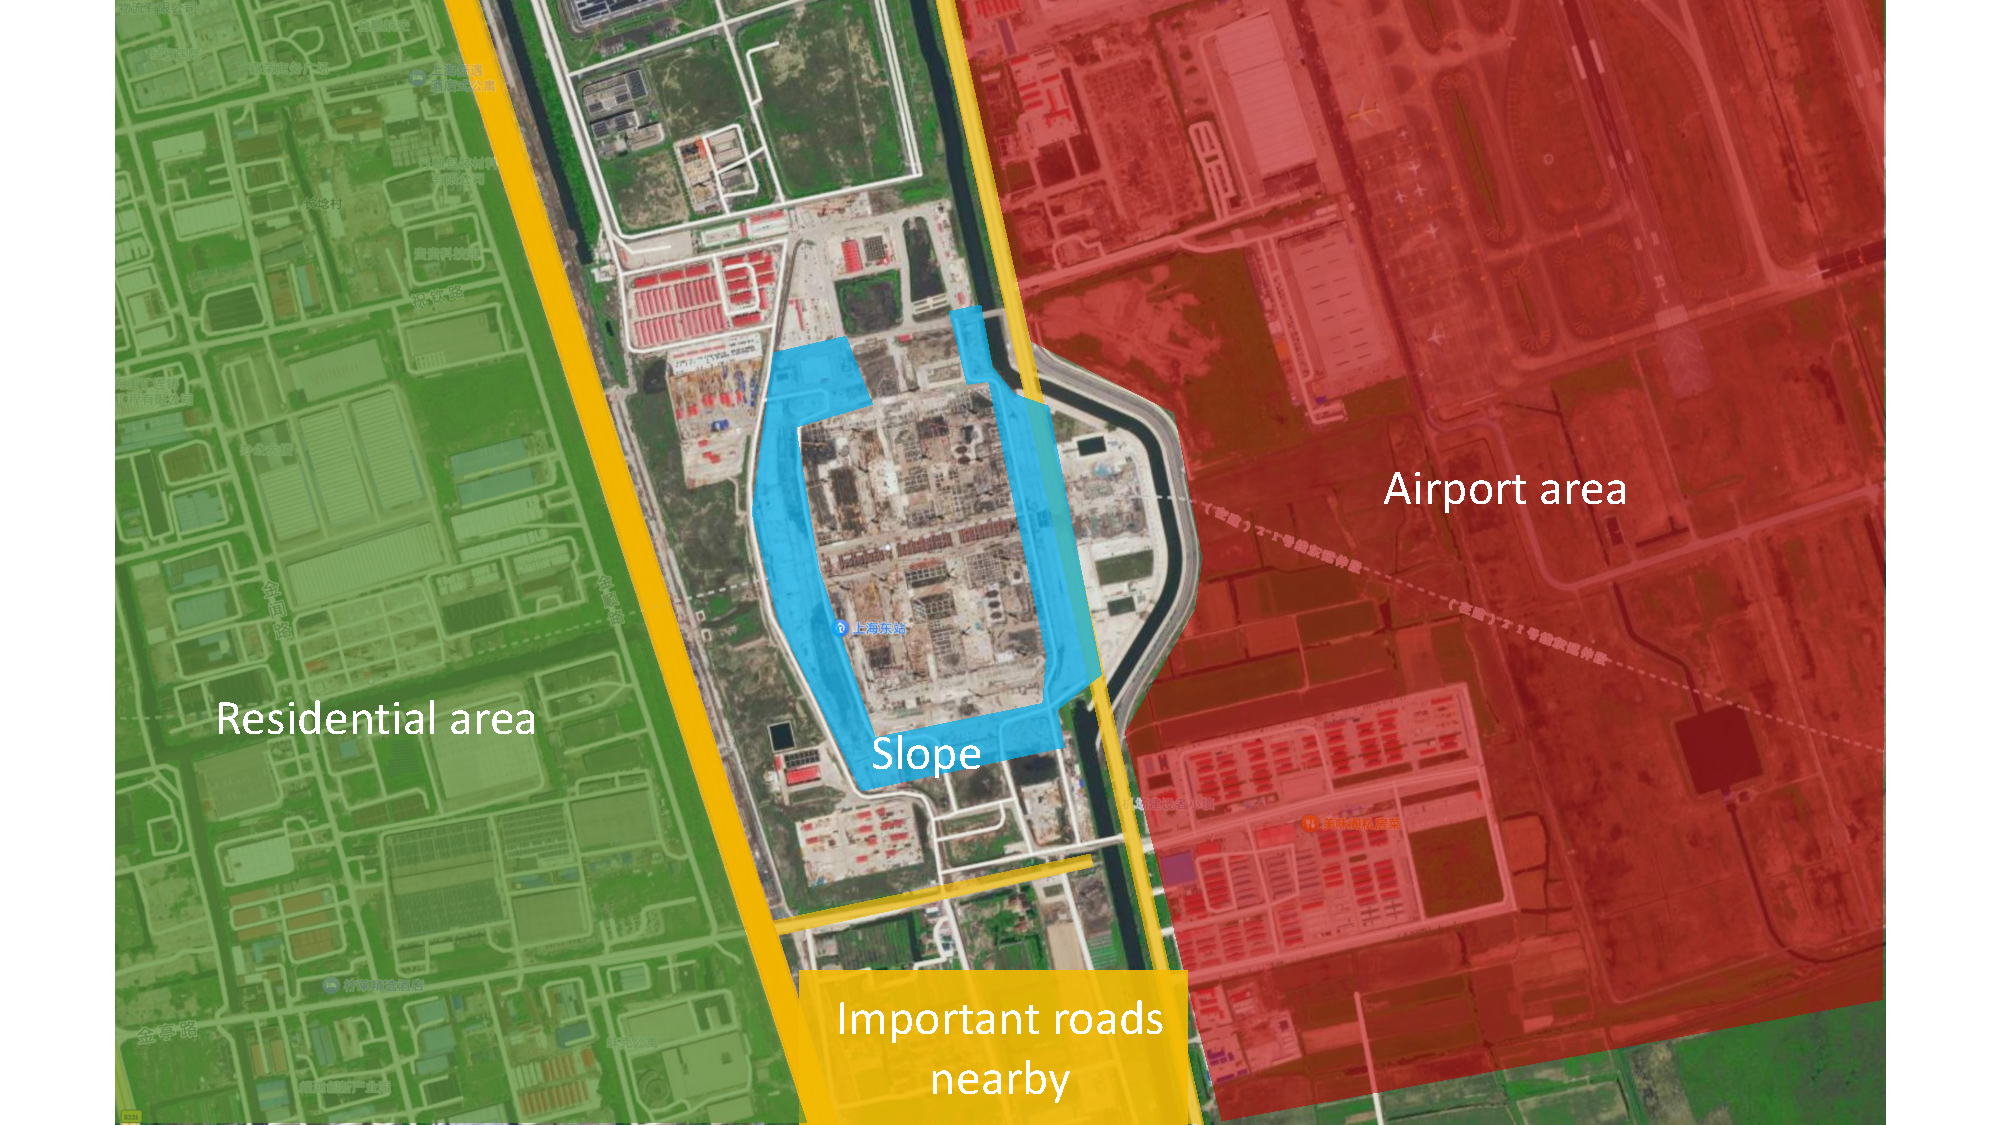
\includegraphics[width=0.9\textwidth]{imgs/Multi_chars.pdf}
    \caption{Complex environment around the excavation project of Shanghai East Railway Station}
    \label{fig:complexEnvironment}
\end{figure}

For example, ground-based monitoring techniques often require manual measurements and are limited by construction, making them unsuitable for large or hard-to-reach areas. Remote sensing technologies, such as optical and radar-based methods, provide broader coverage but may not capture real-time deformations with sufficient accuracy. The inability to monitor large-scale areas continuously and precisely can lead to delayed responses in detecting potential safety hazards or ground instability.
As excavation projects become more complex and the scale of infrastructure grows, the need for comprehensive, real-time, and high-precision monitoring systems has become crucial for ensuring the safety and efficiency of these operations. In response to these challenges, new monitoring solutions integrating multiple technologies are being developed.

\subsection{Technological Needs and Motivation}

The integration of multiple monitoring technologies, specifically combining Space (satellite-based), Air (UAV-based), and Ground (sensor-based) technologies, has emerged as a promising solution. However, to ensure the effectiveness and reliability of these technologies, monitoring systems must comply with established standards and regulations. For instance, in China, the \textit{"Technical Code for Building Excavation Monitoring" (GB 50497-2019)} and \textit{"Code for Design of Foundation Pit Support" (JGJ 120-2012)} provide detailed guidelines on how monitoring systems should be designed and implemented in excavations engineering. These standards emphasize continuous monitoring to detect deformation or instability early and ensure the safety of both the excavation site and surrounding structures.

The integration of UAV, InSAR, and GNSS technologies into a SAG system is highly encouraged by these standards, as they provide complementary data that enhance the overall monitoring capability. By adhering to these national and international regulations, a robust and effective monitoring system can be established, improving the safety and efficiency of large-scale excavation projects.

\subsection{Objectives of the Review and Structure Overview}

This review aims to provide a comprehensive analysis of the current state of Space-Air-Ground (SAG) integrated monitoring technologies, focusing on their applications in large-scale deep excavation engineering. The primary objective is to examine the effectiveness of UAV, InSAR, and GNSS technologies for geotechnical monitoring, and how their integration can provide a more efficient, real-time, and cost-effective solution for excavation monitoring.

The review is organized as follows:

\begin{enumerate}
    \item \textbf{Section 2: Literature Search and Analysis.} This section details the methodology for the literature search and analysis, outlining the databases, search terms, and inclusion criteria used to identify relevant studies. The section further quantitatively analyzes the countries where the literature was published and the number of technological applications. Further, time slicing and evolution analysis were conducted on the key words, and the development characteristics of the technology in different time periods were summarized.
  
    \item \textbf{Section 3: Technology Background and Methods.} This section provides an overview of the principles, technologies, and applications of UAV, InSAR, and GNSS monitoring systems. It highlights the unique capabilities and limitations of each technology in the context of large-scale excavation monitoring.
    
    \item \textbf{Section 4: Data Fusion and Analysis.} This section discusses the integration of UAV, InSAR, and GNSS technologies into SAG systems. It emphasizes the role of data fusion techniques in combining information from multiple sources to improve the accuracy, coverage, and real-time capabilities of monitoring systems. Specific methods for data processing and integration will be explored, including machine learning and statistical approaches.

    \item \textbf{Section 5: Case Studies.} This section highlights case studies where SAG monitoring technologies have been successfully applied in large-scale excavation projects. It showcases the real-world performance and benefits of integrating UAV, InSAR, and GNSS technologies in complex monitoring environments, with an emphasis on practical applications in various geotechnical contexts.
    
    \item \textbf{Section 6: Challenges and Limitations.} This section evaluates the challenges and limitations associated with current monitoring systems, particularly in the context of large-scale deep excavation projects. Topics include the difficulties in real-time data processing, the integration of multi-source data, and the impact of environmental factors on the accuracy of monitoring systems.
    
    \item \textbf{Section 7: Future Directions.} This section presents future directions for research and technological development in the field of SAG integrated monitoring systems. It explores the potential advancements in AI-driven monitoring, automation in data collection, and real-time risk assessment. The section also discusses the future role of machine learning, automated anomaly detection, and predictive modeling in improving monitoring systems for deep excavation projects.
\end{enumerate}

\section{Literature Search and Methodology}

Considering that SAG integrated monitoring technologies are applicable far beyond excavations, the scope of the literature search was expanded to the broader field of geotechnical engineering. When defining search queries in the Web of Science (WoS) database, both the characteristic technologies of SAG monitoring and the common monitoring objectives were taken into account. The final query adopted was:

\begin{quote}
\texttt{TS=("deep excavation" OR "foundation pit" OR Geotechnical) AND
TS=("InSAR" OR "satellite radar" OR UAV OR "drone photogrammetry" OR LiDAR) AND
TS=("monitoring" OR deformation OR safety)}
\end{quote}

Using this query, 687 records were retrieved from Web of Science (WoS) on 26 May 2025, as shown in \autoref{fig:retrieval}, including 13 review articles and 36 dissertations. To further identify the most representative studies, the Chinese Academy of Sciences (CAS) journal ranking system was adopted. After filtering for CAS Zone I-III journals and theses, 522 publications were retained. This classification ensures a baseline research quality while still capturing high-impact papers from both Chinese and international sources \citep{nature:v641}. The distribution of publications by country is illustrated in \autoref{fig:NationalStatistcs}. One review paper that did not specify a project location is excluded from the figure. China contributes the largest number of publications, which is unsurprising given its vast territory and the volume of civil-engineering projects. The United States, Italy, Spain, Canada and the United Kingdom follow; these established industrial nations tend to be more open to the development and early adoption of emerging technologies and thus act as major drivers of innovation.

\begin{figure}[htbp]
    \centering
    
\includegraphics[width=\textwidth]{imgs/advanceSearch.png}
    \caption{Schematic diagram of retrieval results}
    \label{fig:retrieval}
\end{figure}

\begin{figure}[h]
    \centering
    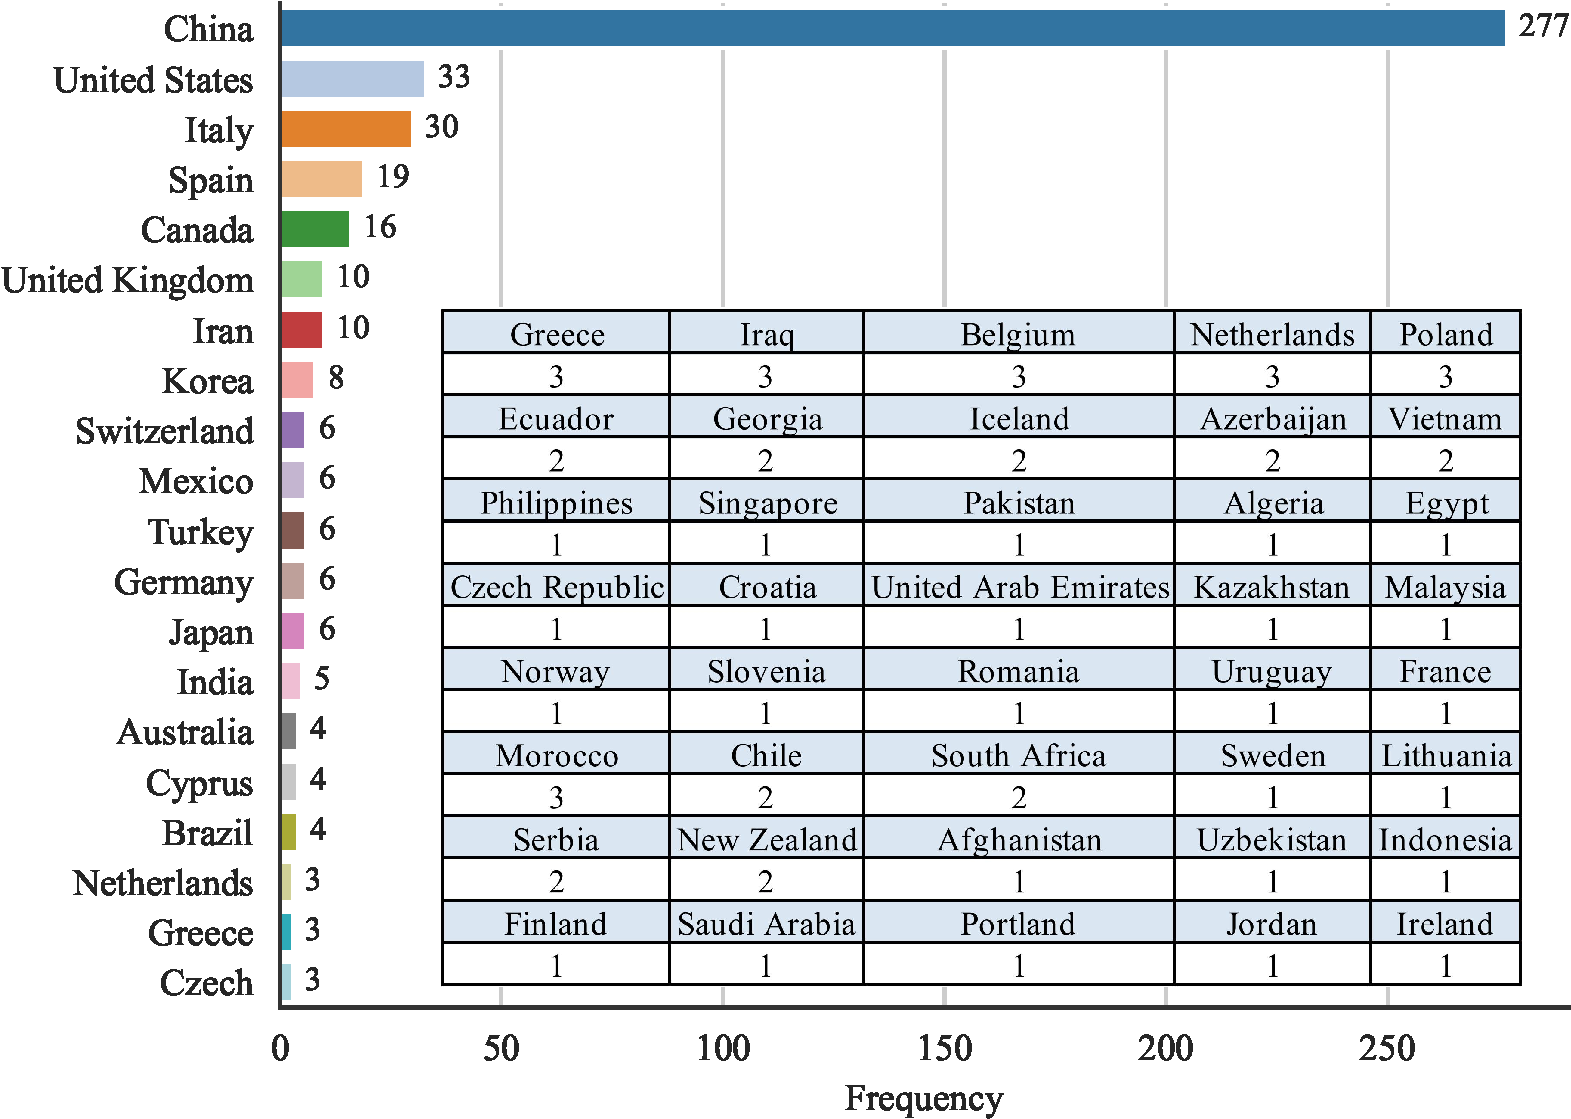
\includegraphics[width=\textwidth]{imgs/countries.pdf}
    \caption{National quantity statistics chart}
    \label{fig:NationalStatistcs}
\end{figure}

To reveal application trends, each paper was annotated with its engineering-project context and year of publication. Project contexts were categorised as follows: \emph{excavation} (deep-pit monitoring), \emph{bridge}, \emph{dam} (hydraulic infrastructure), \emph{flood}, \emph{mining}, \emph{slope}, \emph{tunnel}, \emph{roadbed}, \emph{urban} (urban infrastructure, including suburban airports and railway stations) and \emph{general} (methodological studies without a specific case). Where a paper addressed multiple project types, each type was counted. The relationship between project type and publication year is depicted in \autoref{fig:YearProject}. The number of civil-engineering studies employing SAG monitoring has risen sharply year-on-year, indicating the progressive diffusion of integrated monitoring into structural-safety practice. In terms of project share, \emph{slope}, \emph{dam}, \emph{roadbed}, \emph{urban} and \emph{mining} dominate. Cost and efficiency considerations limit SAG adoption in small-scale excavations, whereas large excavations—often involving \emph{slope}, \emph{roadbed} and \emph{urban} elements simultaneously—demonstrate substantial potential for SAG deployment.

\begin{figure}[htbp]
    \centering
    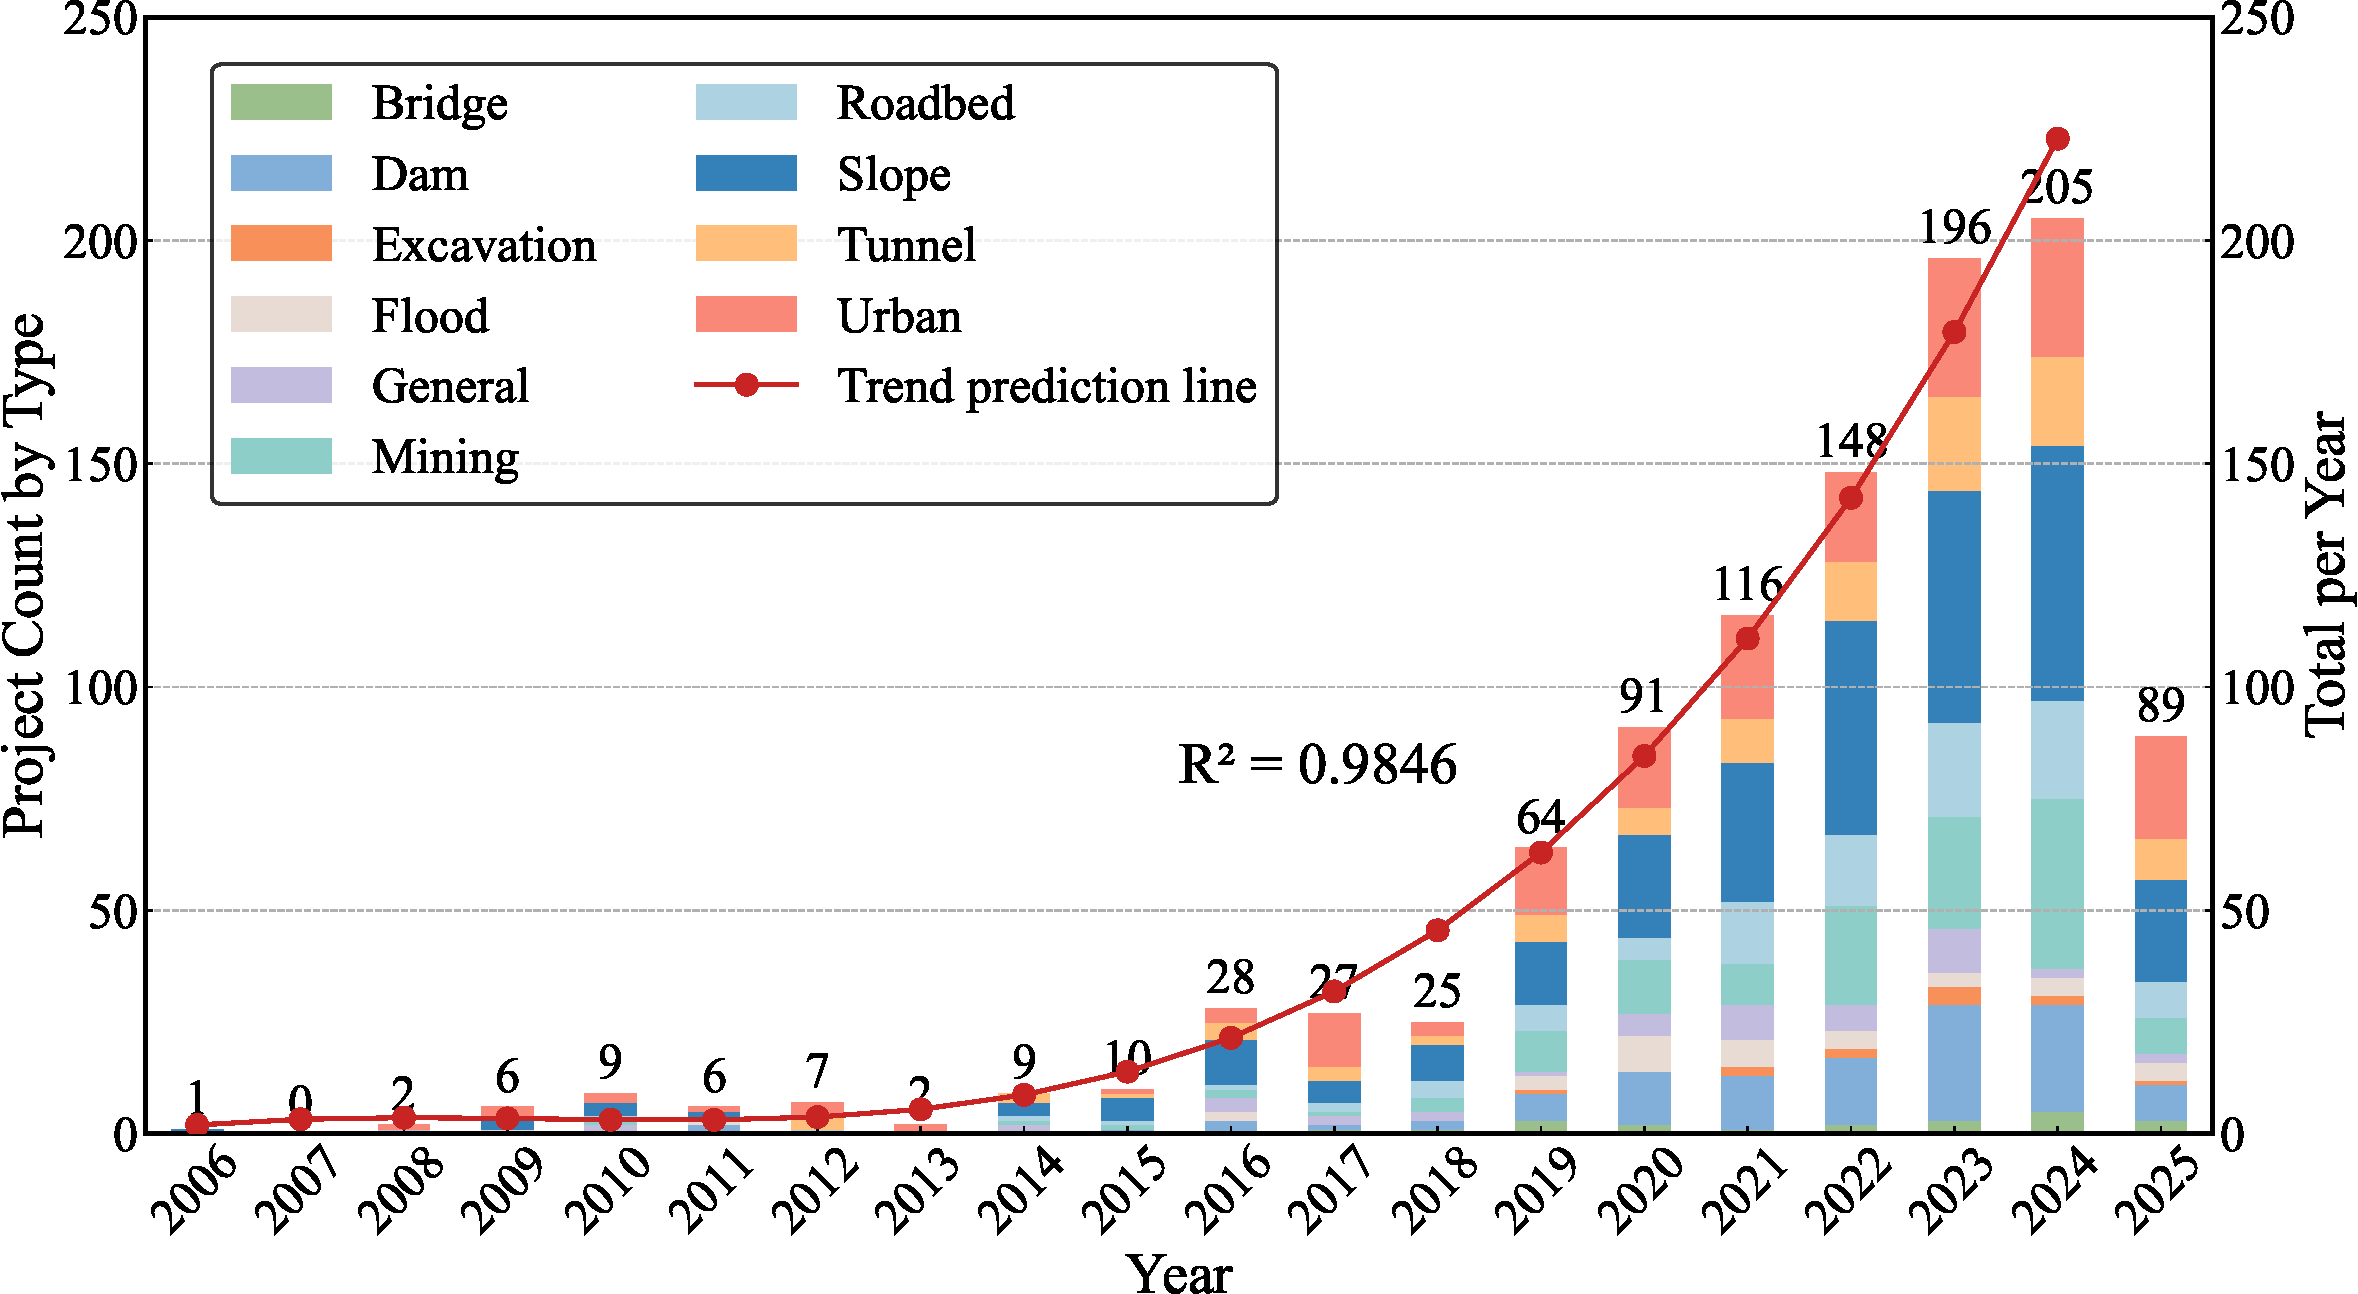
\includegraphics[width=\textwidth]{./imgs/Year_Types.pdf}
    \caption{Statistical chart of year and project types quantity with trend line}
    \label{fig:YearProject}
\end{figure}

To analyze monitoring-technology portfolios, individual techniques were consolidated into broader categories: synthetic-aperture-radar deformation monitoring as \emph{InSAR}; absolute three-dimensional deformation measured by global navigation satellite systems as \emph{GNSS (GPS)}; optical remote-sensing data from UAVs, terrestrial cameras and satellite imagery as \emph{UAV}; laser-point-cloud techniques—including airborne and terrestrial laser scanning—as \emph{LiDAR}; and proximity-sensing methods (ground sensors, ground-based laser radar, etc.) as \emph{Ground}. Because multiple techniques can be combined on a single project, the number of methods used per project type was tallied; results are shown in \autoref{fig:YearTech}. A fifth-order polynomial was fitted to the temporal frequency of each technique. Usage of \emph{LiDAR}, \emph{InSAR} and \emph{UAV} has grown steadily, whereas the frequencies of \emph{Ground} and \emph{GNSS} are stable or slightly declining—likely a consequence of falling sensor costs and the increasing automation of monitoring. Within the SAG framework, \emph{InSAR} and \emph{UAV} constitute the core monitoring solutions.

\begin{figure}[htbp]
    \centering
    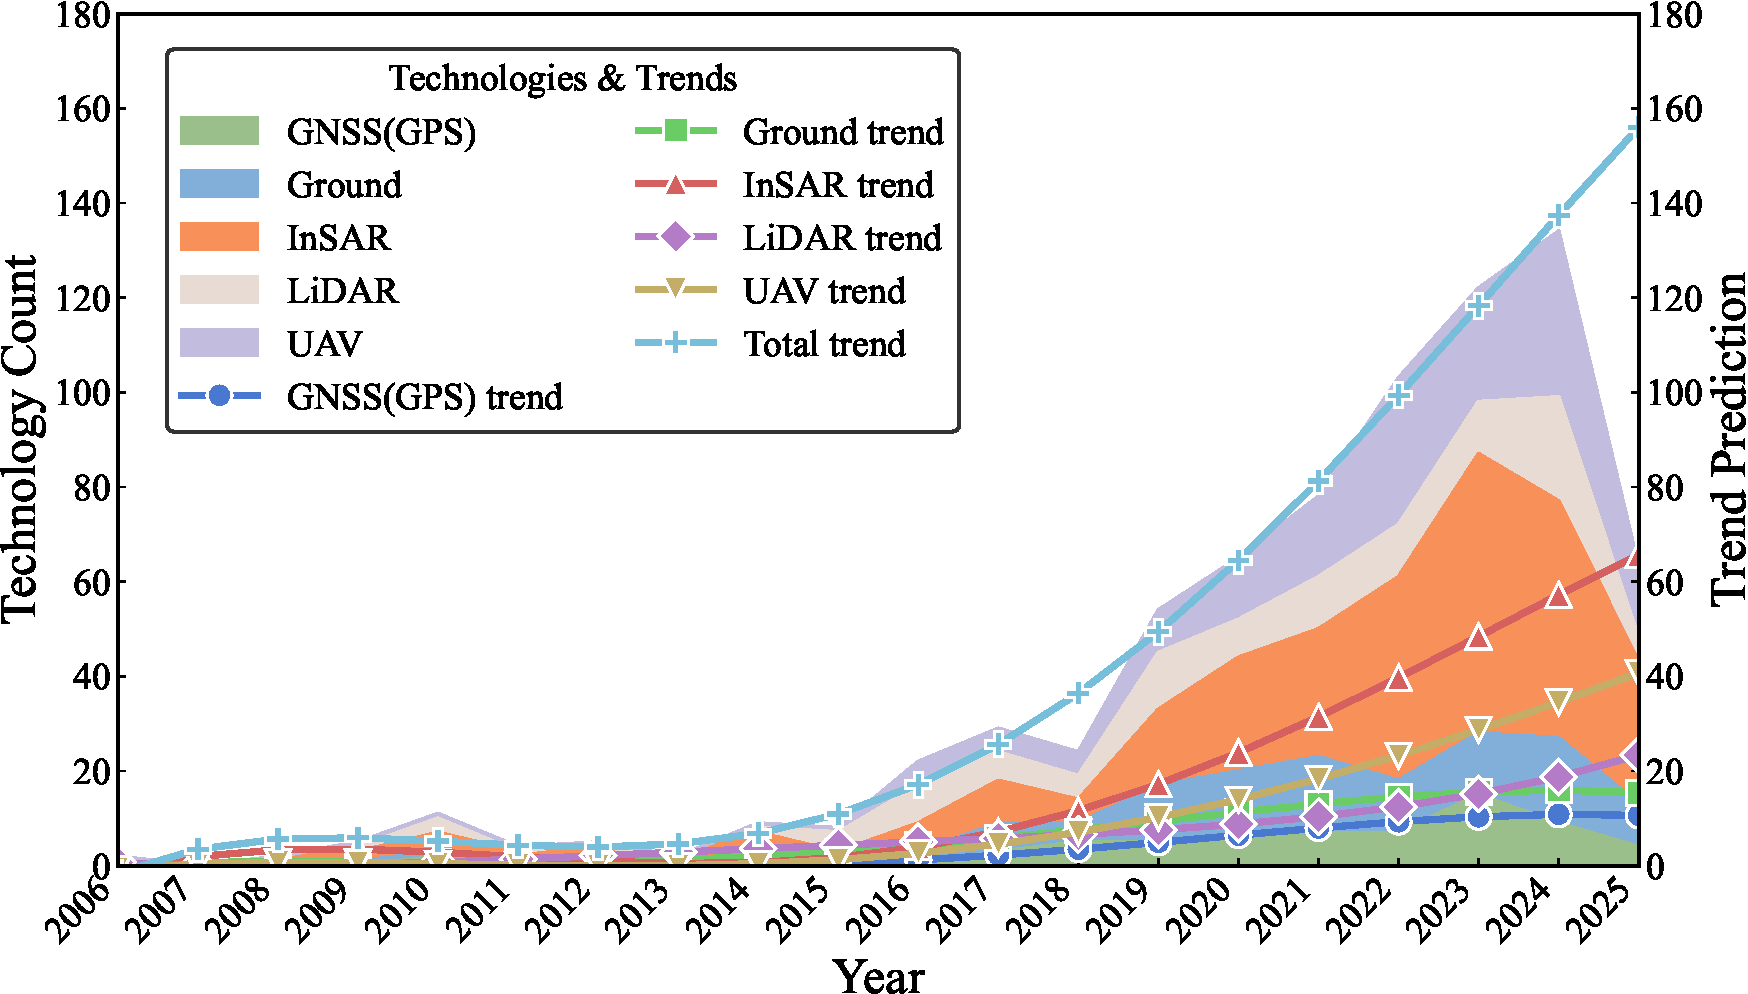
\includegraphics[width=\textwidth]{./imgs/Year_Tech.pdf}
    \caption{Statistical chart of year and technologies quantity with trend line}
    \label{fig:YearTech}
\end{figure}

Keyword co-occurrence analysis is a powerful, systematic method for distilling core themes, research hotspots and evolutionary trajectories from large bodies of literature. To dynamically capture topic evolution and life-cycle stages, we employed a time-slicing approach that traces thematic trajectories and, secondly, applied community-detection algorithms to identify fine-grained hotspots and micro-topics. Following \citep{Lee01042010}, a Python script was developed to perform keyword co-occurrence and community detection in five-year slices. Because the pre-2010 dataset is sparse, three slices were analyzed: 2010-2014, 2015-2019 and 2020-2025. The resulting co-occurrence networks are presented in \autoref{fig:CooccurrenceAnalysis}, and the community-analysis metrics are summarised in \autoref{tab:Co_Nx}. The results confirm that both SAG monitoring technologies and their application fields have advanced and diversified over time. A further quantitative evolutionary analysis extracted technology-related and target-object keywords, with growth trends across time slices listed in \autoref{tab:QuantitativeAnalTab}. Applications of advanced techniques such as \emph{InSAR} and \emph{UAV} have increased year-by-year, expanding from general surface-subsidence observation to dam operation, tunnel construction and smart-city management.

\begin{figure}
    \subfigure[2010-2014·Top 30 keywords·communities=5]{
        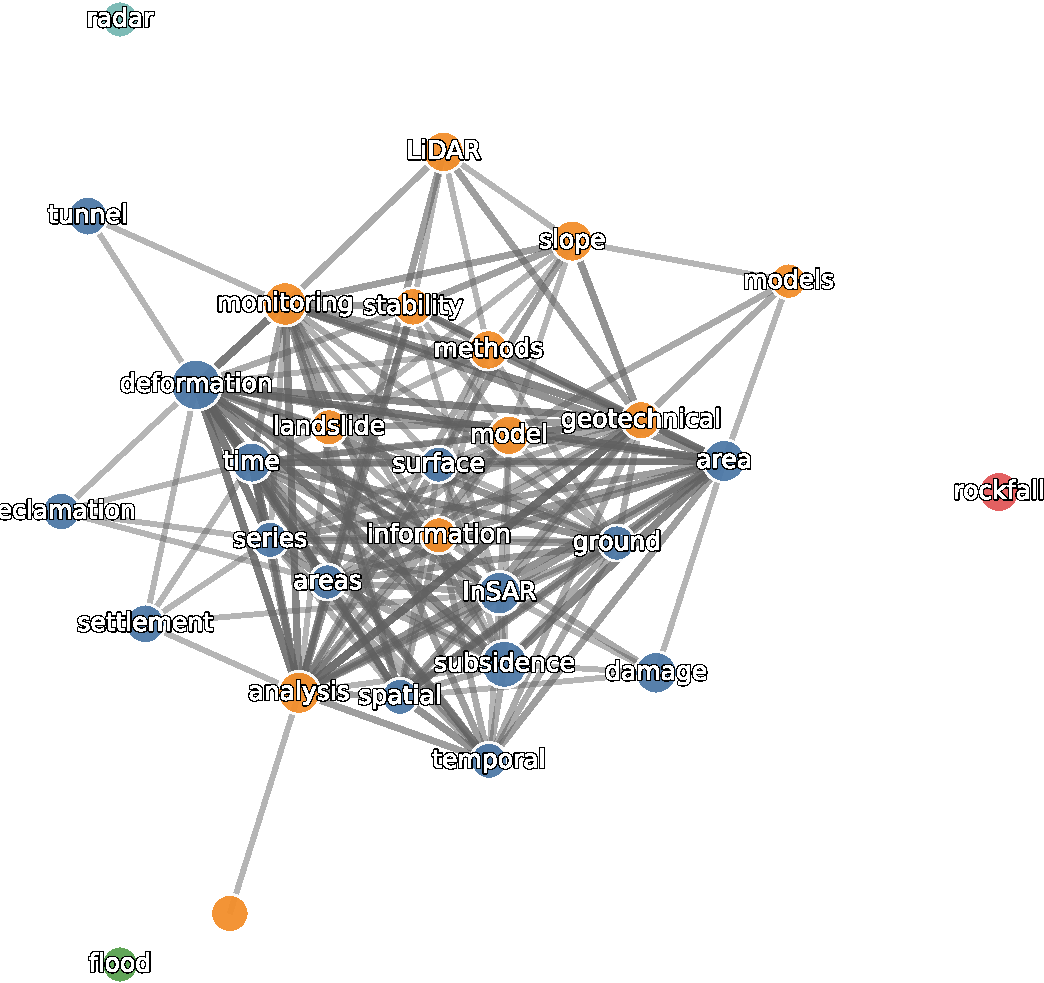
\includegraphics[width=0.5\textwidth]{imgs/keyword_network_2010-2014.pdf}
    }
    \hfill
    \subfigure[2015-2019·Top 30 keywords·communities-3]{
        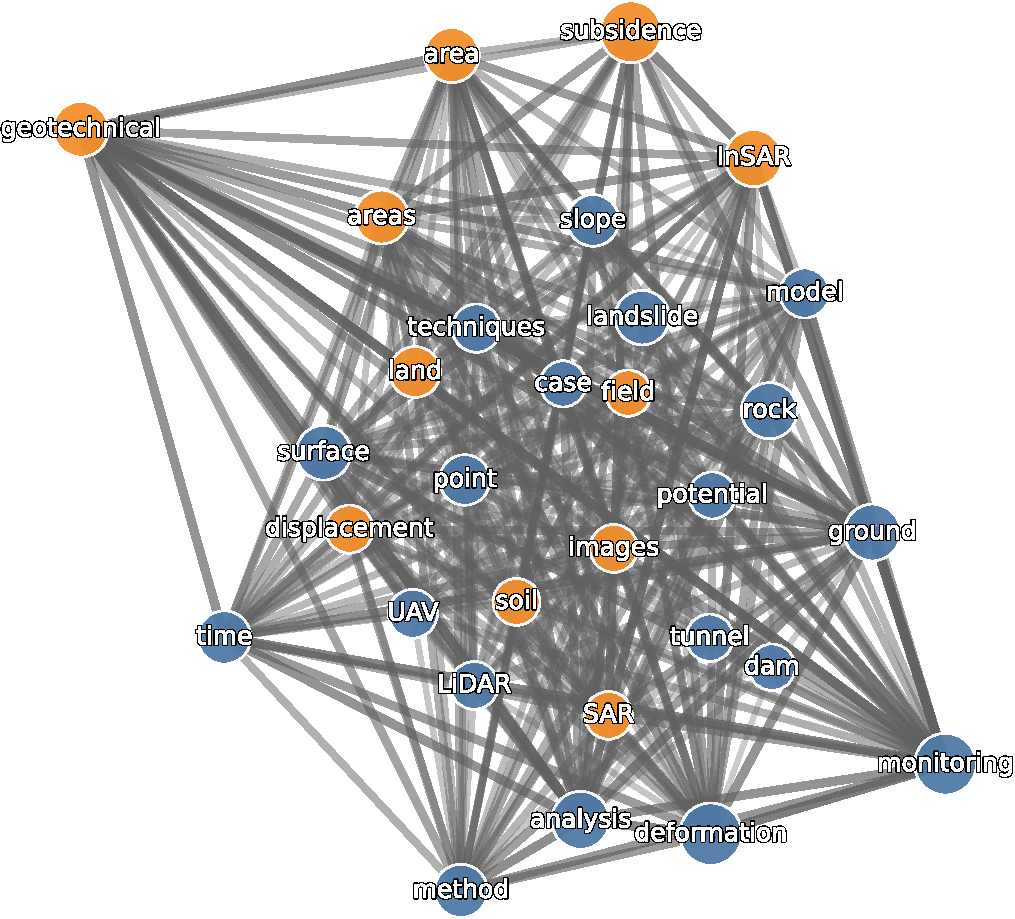
\includegraphics[width=0.5\textwidth]{imgs/keyword_network_2015-2019.pdf}
    }
    \hfill
    \subfigure[2020-2025 ·Top 30 keywords·communities-3]{
        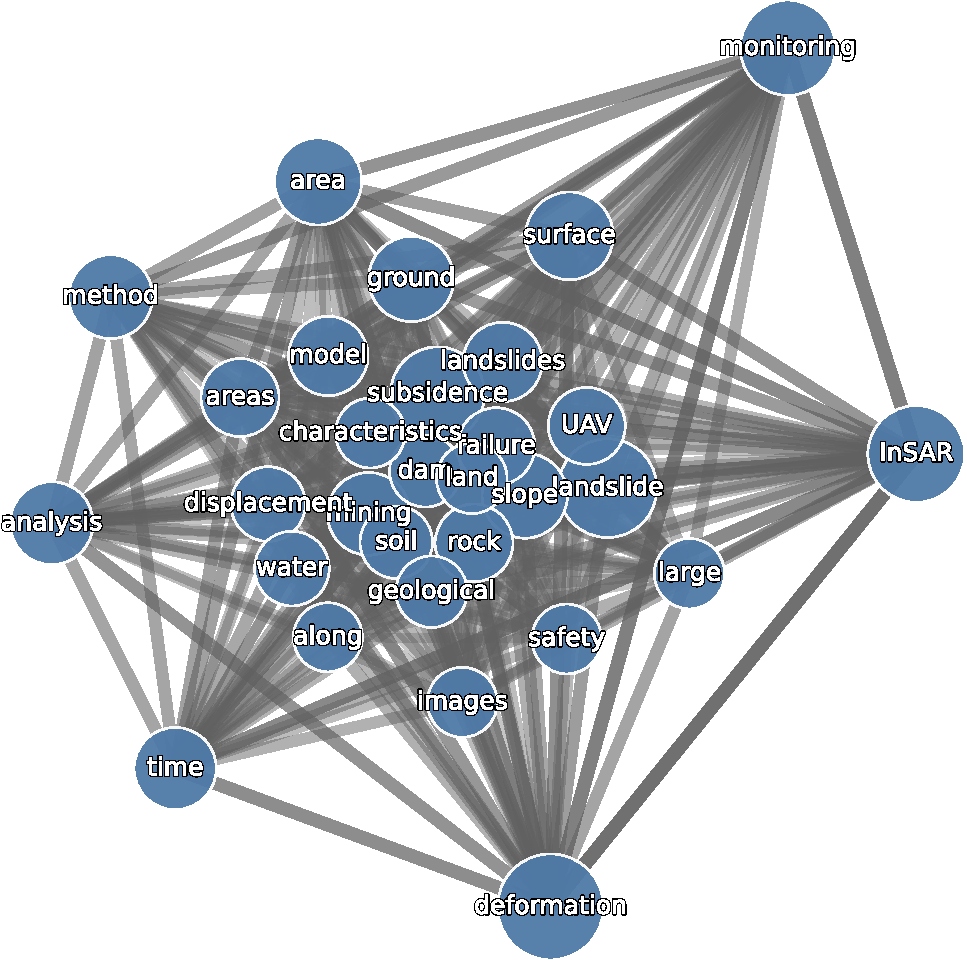
\includegraphics[width=0.5\textwidth]{imgs/keyword_network_2020-2025.pdf}
    }
    \caption{Co-occurrence analysis diagram of community identification keywords in different time periods}
    \label{fig:CooccurrenceAnalysis}
\end{figure}

\begin{table}[htbp]
    \centering
    \caption{Temporal evolution of the keyword co‐occurrence network}
    \label{tab:Co_Nx}
    \begin{tabular}{p{4em}p{5em}p{4em}p{4em}p{4em}p{18em}}
        \toprule
        \textbf{Period} & \textbf{Publications} & \textbf{Nodes} & \textbf{Edges} & \textbf{Communities} & \textbf{Key observations} \\
        \midrule
        2010--2014 & 22  & 25 & 166 & 3 & The early network is relatively sparse; topics such as \textit{LiDAR}, \textit{tunnel} and \textit{settlement} remain largely independent, exhibiting a multi-core structure. \\
        
        2015--2019 & 92  & 25 & 287 & 1 & With the surge in publications, connections among core high-frequency terms become markedly denser, community boundaries blur, and a single dense mega-cluster forms; the themes "monitoring-data-deformation" are tightly coupled and SAG spreads rapidly in multiple scenarios. \\
        
        2020--2025 & 403 & 25 & 300 & 1 & Node degree and size continue to rise, and the network approaches a "highly integrated" configuration. New terms such as \textit{UAV}, \textit{InSAR}, and \textit{mining} enter the Top-25 list but are rapidly absorbed into the main community, indicating strong cross-fertilization and convergence of the thriving research topics. \\
        \bottomrule
    \end{tabular}
\end{table}

\begin{table}[htbp]
  \centering
  \caption{Quantitative analysis table of keyword co-occurrence}
    \begin{tabular}{cccccc}
    \toprule
    \textbf{Keyword} & \textbf{2010-2014} & \textbf{2015-2019} & \textbf{Growth\_2015-2019} & \textbf{2020-2025} & \textbf{Growth\_2020-2025} \\
    \midrule
    \textbf{InSAR} & 23    & 70    & 204.3\% & 582   & 731.4\% \\
    \textbf{slope} & 22    & 48    & 118.2\% & 374   & 679.2\% \\
    \textbf{UAV} & 0     & 38    & -     & 232   & 510.5\% \\
    \textbf{dam} & 10    & 36    & 260.0\% & 211   & 486.1\% \\
    \textbf{subsidence} & 35    & 101   & 188.6\% & 562   & 456.4\% \\
    \textbf{displacement} & 7     & 39    & 457.1\% & 212   & 443.6\% \\
    \textbf{ground} & 13    & 74    & 469.2\% & 374   & 405.4\% \\
    \textbf{tunnel} & 18    & 35    & 94.4\% & 166   & 374.3\% \\
    \textbf{infrastructure} & 4     & 27    & 575.0\% & 82    & 203.7\% \\
    \textbf{urban} & 5     & 33    & 560.0\% & 70    & 112.1\% \\
    \bottomrule
    \end{tabular}
  \label{tab:QuantitativeAnalTab}
\end{table}

To further analyze and synthesize the application methodologies of SAG technology within excavation engineering monitoring, thereby aiming to provide robust guidance for future implementations, the subsequent sections will pursue several key objectives. A comprehensive review of pertinent global and national standards and codes concerning monitoring parameters and precision control requirements for excavation projects will be presented. Additionally, SAG monitoring methodologies, identified through an extensive literature survey, will be detailed. The salient characteristics of diverse monitoring technologies will be analyzed. Finally, established approaches for maximizing the utility of heterogeneous, multi-source data acquired through an integrated monitoring framework will be summarized.

\section{Technology Background and Methods}

\subsection{Global regulations for Excavation Engineering Monitoring}

Modern excavation projects are increasing in scale, depth, and proximity to critical infrastructure, elevating risks and environmental control challenges, thereby driving demand for advanced monitoring technologies. Early regulations focused on basic safety and manual quality checks, but the advent of automation (e.g., total stations, sensors) in the late 20th/early 21st centuries led to codes incorporating requirements for automated data acquisition, including precision, installation, and initial processing. Deep excavations, distinct from other geotechnical projects due to short construction cycles, rapid disaster onset, and on-face monitoring locations, demand specific monitoring capabilities:

\begin{enumerate}
    \item Timeliness: Rapid onset of instability necessitates second-to-minute sampling and automated data transmission.
    \item Spatial Density: High sensor density (e.g., 10-30 m grid) is crucial; for instance, the Shanghai East Railway Station project required 5 m density due to its importance and complexity.
    \item Construction Interference: Frequent site activities and on-face sensor placement mean sensors often record impact data and risk damage.
\end{enumerate}

SAG integrated monitoring in excavations often combines space-ground synergy (e.g., InSAR for settlement) and air-ground synergy (e.g., UAV photogrammetry for deformation). Air-borne monitoring offers wide, long-duration surveillance, while space-borne methods provide precise, automated mapping. The ISO 18674 series ('Geotechnical monitoring by field instrumentation') \citep{ISO18674-1:2015,ISO18674-2:2016,ISO18674-3:2017} is a core global guide, with ISO 18674-1 establishing unified terminology and quality control frameworks. Supporting standards like ISO/IEC Guide 99 \citep{JCGM200:2012} (metrology) and IEC 60529 \citep{IEC60529:2013} (IP ratings) contribute to a comprehensive standardization ecosystem.

Global regulations for intelligent excavation monitoring vary; some regions have specific guidance for automation, while others use general codes. Eurocode 7 (EN 1997) \citep{EN1997-1:2024} is Europe's core geotechnical design standard, with Part 4 covering supervision, monitoring, and maintenance. A key concept is the Observational Method (OM), allowing design adjustments based on monitoring, subject to strict requirements like defining performance limits, assessing behaviors, planning, instrument response times, and rapid response protocols for hazards.

In the UK, BS 5930 \citep{BS5930:2015+A1:2020} and CIRIA C661 \citep{CIRIA_C661:2008}, derived from EN 1997, address monitoring. CIRIA C661 introduces 'intelligent monitoring' for concrete structures (automated assessment of condition and deterioration for predicting remaining life). The updated CIRIA R185 ('The Observational Method in geotechnical engineering') \citep{CIRIA_R185:1999} is vital for modern OM practice, expected to integrate technologies like real-time feedback.

German geotechnical design, historically using DIN standards (global factor of safety), now aligns with Eurocode 7's limit state design. DIN 1054 \citep{DIN1054:2021-04} details the Observational Method, mandating behavior prediction, measurement-based control, result comparison, and critical situation responses.

The U.S. excavation monitoring framework is diverse, involving OSHA (safety), FHWA (guidelines), USACE (manuals), and ASTM (standards). FHWA's 1998 'Geotechnical Instrumentation Reference Manual' \citep{Dunnicliff:1998:FHWA} detailed monitoring plans and data handling. USACE's EM 1110-2-1908 \citep{USACE_EM1110-2-1908:2020}, though for dams, offers valuable insights on ADAS, data management, and new technologies (fiber optics, TDR) relevant to excavations. The U.S. lacks a unified national standard for intelligent excavation monitoring, with developments being largely project-driven or research-oriented rather than mandatory regulations.

The Canadian Foundation Engineering Manual (CFEM), fifth edition \citep{CFEM:2023}, includes a chapter on 'Geotechnical Instrumentation and Monitoring.' It details instrument principles and selection for monitoring excavation support deformations, groundwater pressure, support system forces, earth pressure, and environmental impacts, emphasizing systematic plans, ADAS, and data interpretation within a framework of design verification, construction control, and risk management (including OM). However, it focuses on conventional ground-based methods.

China's excavation monitoring regulations blend national standards and complementary local codes. National standards like JGJ 311 \citep{JGJ311:2013} (safety) and GB 50497 \citep{GB50497:2019} (technical methods, quality control) provide a base. Local standards are often more advanced in intelligent monitoring; e.g., Wuhan's regulations \citep{DB4201_T738:2025} cover automation details, and Fujian's standard \citep{DBJ_T13-416:2024} addresses AI in visual/laser measurement and BIM/CAD integration. Local codes offer detailed methodologies for equipment and quality control.

Singapore's Building and Construction Authority (BCA) regulates excavations via guidelines, requiring impact assessments and defining monitoring levels (Alert, Work Suspension, and Action Levels under the 'Rigorous Approach' with intensive monitoring for settlements, tilt, and cracks). Recent measures, like mandatory video surveillance on sites over SGD 5 million for 24/7 monitoring and safety, promote advanced monitoring technologies.

Japanese geotechnical standards, mainly from the Japanese Geotechnical Society (JGS) with MLIT guidelines, include methods like surface extensometer \citep{JGS1725:2012} and borehole inclinometer measurements \citep{JGS3722:2012} for deformation monitoring, but lack comprehensive SAG integration. Monitoring practices depend more on corporate/research innovation and project-specific applications than top-level mandates.

Australian excavation monitoring involves Australian Standards (AS), Australian Geomechanics Society (AGS) guidelines, and state/territory WHS regulations. AS 4678 \citep{AS4678:2002} ('Earth-retaining structures') notes monitoring for design verification. The AGS's 2023 'Guideline on Planning for Data Management for Geotechnical Instrumentation and Monitoring Projects' \citep{AGS:DataManagementGuide2023} focuses on data management to support decisions, primarily for ground-based methods, reflecting an industry consensus on enhancing data value.

Global excavation monitoring is shifting towards automation, intelligence, and SAG integration. Disparities exist in regulatory maturity and adoption of multi-source data integration and AI, with some Asian regions (e.g., parts of China) leading in relevant technical standard development. The characteristics of sky-based, air-based, ground-based technologies and the applicability of different technologies to excavation projects are summarized as the following paragraphs.

\subsection{Space-based Monitoring}

In civil engineering, space-based monitoring mainly selects InSAR, optical remote sensing and GNSS measurement, which implement different effects through different working mechanisms \citep{KOOHMISHI2024105378}.

\subsubsection{InSAR}

As an active microwave remote sensing system, Synthetic Aperture Radar (SAR) generates images of the ground surface by transmitting microwave pulses and recording the backscattered signals. This active capability ensures operation independent of lighting conditions and allows for all-weather observation due to the penetration of microwave signals through clouds, fog, and light rain. InSAR technology leverages the phase information within complex SAR images acquired from the same area on at least two separate occasions \citep{8977523}. The fundamental principle involves calculating the phase difference, $\Delta \phi$, which is directly proportional to the radar signal path difference $\delta r$ between acquisitions $\Delta\varphi=\frac{4\pi}{\lambda}\delta r$, where $\lambda$ is the radar wavelength), thereby capturing precise details about surface topography and deformation \citep{752187}. Nevertheless, the calculated phase difference comprises contributions from numerous sources, and the accurate extraction of the deformation signal from this composite phase remains a critical technical aspect of InSAR deformation measurement \citep{HU20141}. 

Differential InSAR (DInSAR) is used to extract the information of ground surface deformation, after which the terrain phase derived from an external Digital Elevation Model (DEM) is subtracted to reveal the surface deformation between the acquisitions \citep{GIUDICEPIETRO2024104060}. Nevertheless, the accuracy of a single DInSAR interferogram is subject to several limitations, including atmospheric delay effects (due to tropospheric water vapor, temperature, and pressure variations), temporal decorrelation, spatial decorrelation, and changes in surface cover, all of which can result in significant errors \citep{SAMSONOV2024114049}. Permanent-Scatterer InSAR (PS-InSAR) is proposed to reduce the influence of atmospheric delay effect and spatial decorrelation by establishing the phase difference model between adjacent permanent scatterers \citep{ferretti1999permanent, ferretti2002permanent}. To solve the problem of sparisty of permanent scatterers, Small Baseline Subset InSAR (SBAS-InSAR) is to proposed by ubsing distributed scatterers which can keep correlation in a short time \citep{berardino2002new}. And now, to further increase the density and accuracy of scatterers, PS-InSAR and Distributed-Scatterer InSAR (DS-InSAR) are mixed by adding more random micro-scatterers, and a new algorithm is proposed named \textit{SqueeSAR} \citep{Ferretti2011SqueeSAR, MontiGuarnieri2008TargetStatistics, samiei2016phase, even2018insar}. In addition, Corner Reflector InSAR (CRInSAR) can be deployed in the monitoring field as stable permanent scatterers to improve the monitoring accuracy significantly \citep{Luzi2022ActiveReflector, Garthwaite2017CRDesign}. As the two most widely adopted InSAR techniques, PS-InSAR and SBAS-InSAR fall under the umbrella of Time-Series InSAR methods. By processing extensive time series datasets (typically exceeding 15-20 SAR scenes), these techniques effectively mitigate errors \citep{TimeSeriesInSAR}. Regarding applicability, PS-InSAR is better suited for urban engineering project monitoring, whereas SBAS-InSAR is generally preferred for monitoring projects in non-urban environments.

InSAR technology is extensively employed for monitoring excavation projects. As an example, a excavation project on the reclaimed land of Incheon Songdo utilized PS-InSAR technology. Employing 39 scenes of Sentinel-1b C-band descending IW mode SLC imagery acquired from August 2015 to January 2018, PS points were identified using the amplitude dispersion index method, followed by phase unwrapping and error correction. A total of 107,414 PS points were identified across the entire Songdo area, with annual subsidence rates reaching 2 cm/yr in some areas. Within the excavation construction area, PS-InSAR detected significant subsidence, and ground settlement gauge measurements (approximately 8mm settlement within the first week of construction) validated the subsidence trend monitored by InSAR. In a deep excavation project in Oslo, Norway, PS-InSAR was utilized to evaluate the impact of excavation on adjacent buildings. By comparing the InSAR measurement results with data from traditional monitoring methods (such as inclinometers), it was found that high-resolution InSAR measurements were more reliable in assessing the response of adjacent buildings to the excavation \citep{ritter2021insar}. In a ground subsidence monitoring project along the Shanghai metro network, PS-InSAR and machine learning methods were used to analyze 40 scenes of Sentinel-1A ascending SAR imagery acquired from May 2016 to December 2017. Based on subsidence magnitude, a risk matrix was constructed, and five risk levels were delineated, leading to the identification of high-risk areas along the metro network \citep{chen2023integration}. In excavation engineering, InSAR technology is primarily applied for monitoring key indicators such as ground subsidence and the horizontal and vertical deformation of adjacent structures, notably enabling deformation monitoring over extensive areas, with measurement precision typically at the 1-2mm level. The workflow for InSAR-based monitoring of ground subsidence and building tilt is illustrated in the \autoref{fig:InSARMonitoring}.

\begin{figure}[h]
    \begin{center}
        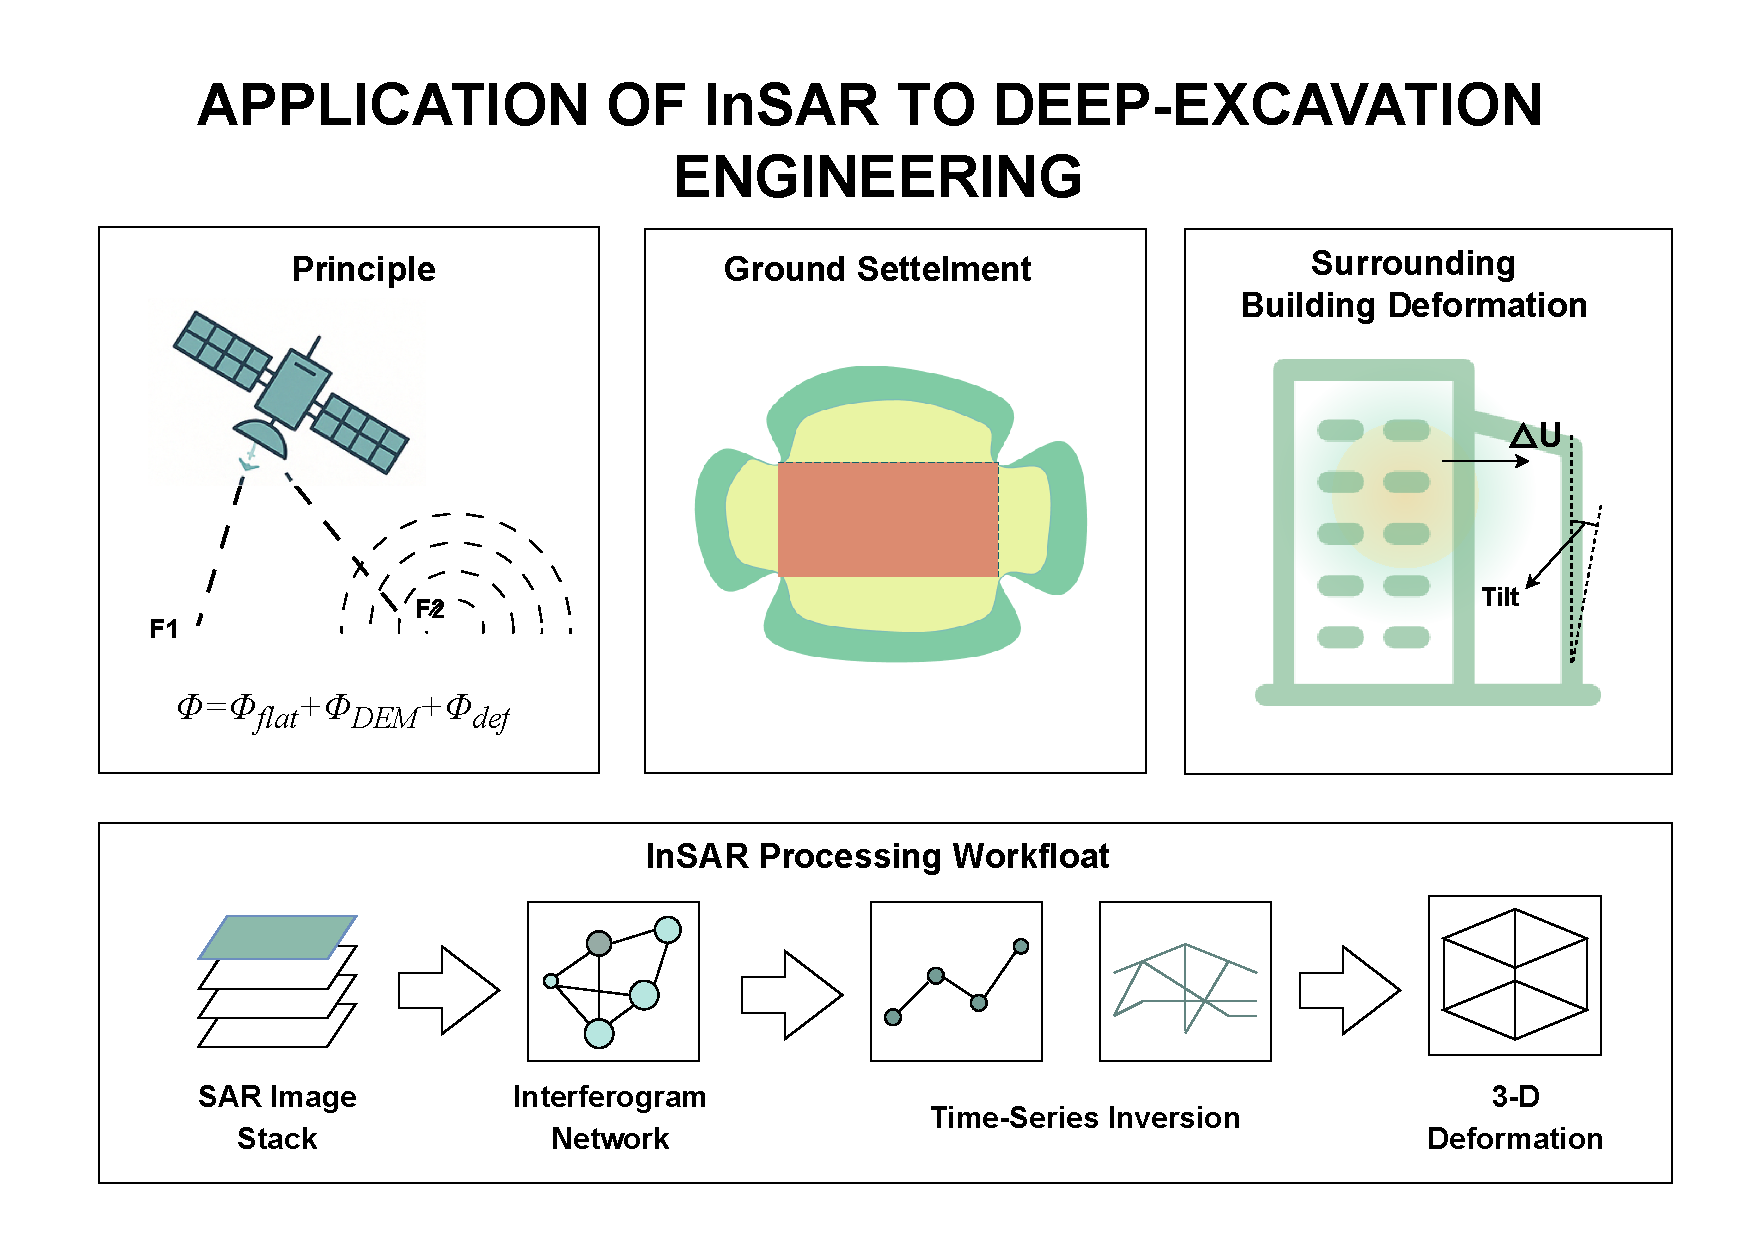
\includegraphics[width=0.8\textwidth]{imgs/InSAR_Flow.pdf}
        \caption{The workflow of InSAR to monitroing the excavation engineering}
        \label{fig:InSARMonitoring}
    \end{center}
\end{figure}

\subsubsection{Optical Remote Sensing}

Optical satellite remote sensing is a technology that utilizes optical sensors carried on satellite platforms to receive information from the sun's reflection off ground objects or their own emitted thermal radiation, and converts this information into image data. It plays a significant role in the field of engineering monitoring, especially in macro-scale and land cover change monitoring. Optical remote sensing primarily includes multispectral and hyperspectral remote sensing. Multispectral remote sensing typically acquires data in several (3-10) relatively wide spectral bands, such as the common blue, green, red, and near-infrared bands. Hyperspectral remote sensing, on the other hand, can acquire data in tens to hundreds of continuous and narrow spectral bands, offering higher spectral resolution. This enables hyperspectral remote sensing to capture more detailed spectral characteristics of ground objects, thereby facilitating more accurate material identification, component content inversion, etc. \citep{colomina2014unmanned}. In civil engineering monitoring, multispectral technology is often used for macroscopically observing surface information, conducting rapid mapping or landform comparison, rather than precise millimeter-level deformation measurement \citep{joshi2016review, casas2024remote}. Optical remote sensing has several key accuracy indicators, including:

\begin{enumerate}
\item Spatial Resolution: The resolution of some commercial satellites can reach sub-meter levels, such as high-resolution satellites like Pléiades Neo, WorldView, and GeoEye with 30cm accuracy.
\item Geometric Accuracy: Refers to the degree of agreement between the position of ground objects in the image and their true geographical coordinates. Correction based on ground control points or high-precision DEM is required, and sub-meter accuracy can be achieved.
\item Temporal Resolution: Refers to the frequency at which the satellite repeatedly observes the same location. High-resolution satellites have a revisit period of several days or tens of days, while medium and low-resolution satellites can observe daily or even more frequently.
\item Spectral and Radiometric Resolution: Spectral resolution determines the ability to distinguish between different ground objects, while radiometric resolution represents the grayscale levels and detail expression capability of the image through the number of bits.
\end{enumerate}

Optical remote sensing is mainly used in civil engineering monitoring for the stability monitoring of dams and slopes. For excavation projects, it can be used for the slope stability monitoring of large-scale deep excavations, such as the multi-level retaining slopes of the Shanghai East Station building in China, as shown in the \autoref{fig:complexEnvironment}.

\subsubsection{GNSS}

GNSS is a measurement technology that measures the displacement of a point, utilizing satellites, providing Positioning, Navigation, and Timing (PNT) services globally. Currently, the major operational systems include BeiDou (China), GPS (United States), GLONASS (Russia), and Galileo (European Union). The primary positioning methods of GNSS are absolute positioning and differential positioning. The former employs a single receiver, while the latter uses two or more receivers for data processing to significantly enhance accuracy. Differential positioning methods are predominantly used in civil engineering monitoring, where a reference station is deployed at a fixed point, and multiple monitoring stations are set up at the points of interest, as shown in the \autoref{fig:GNSSMonitoring}

\begin{figure}
    \centering
    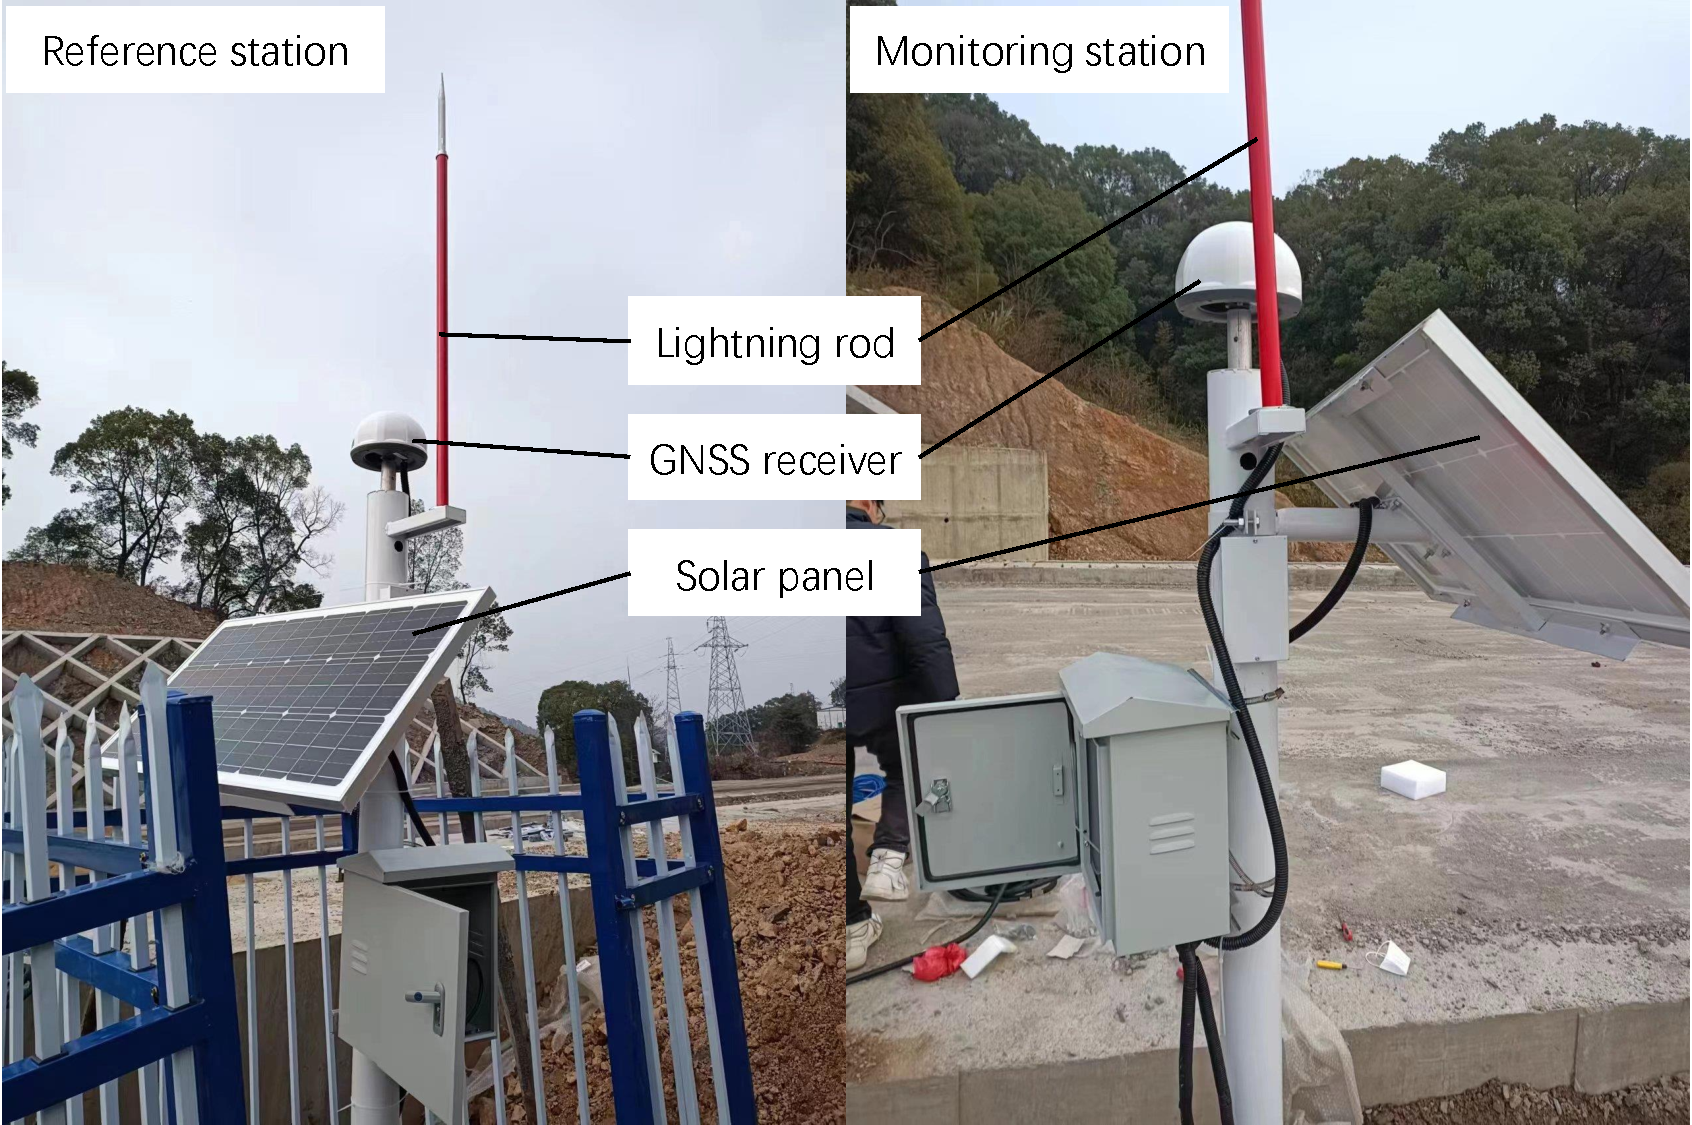
\includegraphics[width=0.8\textwidth]{imgs/GNSSMonitoring.pdf}
    \caption{The actual GNSS monitoring situation of a slope project in Jiangxi Province, China}
    \label{fig:GNSSMonitoring}
\end{figure}

Some new processing techniques or advanced receiving systems have been developed to improve GNSS monitoring accuracy or reduce monitoring costs. Real-Time Kinematic (RTK) is a differential GNSS technique based on carrier phase measurements. By using correction coordinates calculated from a base station with known precise coordinates to correct the observation data obtained by the monitoring station via differencing, common errors such as satellite clock errors, receiver clock errors, ephemeris errors, and atmospheric delays under short baseline conditions can be eliminated or significantly weakened \citep{huang2023gnss, shen2019review}, but it requires the coordinates of the base station to be accurate and fixed. As it is difficult to find fixed points near large engineering areas, Network RTK (Network RTK) was proposed to solve the problem of difficulty in setting up fixed base stations, by establishing a network composed of at least three Continuously Operating Reference Stations (CORS) to replace the fixed base station. These CORS stations transmit their observation data in real-time to a central server. The server sends correction data to the receiving terminal via mobile networks. Users do not need to deploy RTK facilities and only need to subscribe to the service, but its operation relies on a stable wireless network \citep{weng2021improving}. To achieve precise positioning anywhere globally, Precise Point Positioning (PPP) was proposed. It utilizes undifferenced observation data from a single GNSS receiver, correcting satellite positions and time references based on high-precision satellite orbit and clock products. However, PPP technology requires several minutes or even tens of minutes for initialization before use \citep{knoop2017lane}. Static and rapid static differential positioning utilize at least two receivers (one base station, one or more monitoring stations) to synchronously observe a set of satellites. By using carrier phase differencing techniques to accurately determine baseline vectors, it is currently the positioning method with the highest accuracy and is faster \citep{CARDELLACH20082927, zangenehnejad2021gnss}. To reduce the complexity or cost of equipment deployment, some projects adopt single receivers for direct displacement measurement, such as using VADASE (Variometric Approach for Displacements Analysis Stand-Alone Engine) to monitor seismic activity \citep{shen2019review}, or developing low-cost receiver chips based on MEMS technology to achieve low-cost automated monitoring network construction \citep{marut2024affordable}, etc. The basic principles, accuracy, limitations, advantages, and disadvantages of different GNSS techniques are shown in the \autoref{tab:GNSSCompare}. Since GNSS is deployed at the points to be measured, GNSS is also often classified under ground-based monitoring.

\begin{landscape} % 如果表格需要横向显示
    \begin{longtable}{p{5em}p{8em}p{7em}p{5em}p{7em}p{7em}p{6em}p{12em}}
        \caption{Comparison of GNSS Techniques} \label{tab:GNSSCompare} \\
        \toprule
        Technique Name & Basic Principle & Typical Accuracy (Horizontal/Elevation) & Convergence Time & Operating Range/Baseline Limitation & Infrastructure Requirements & Main Advantages & Main Limitations \\
        \midrule
        \endfirsthead 

        \multicolumn{8}{c}
        {{\bfseries \tablename\ \thetable{} -- continued}} \\
        \toprule
        Technique Name & Basic Principle & Typical Accuracy (Horizontal/Elevation) & Convergence Time & Operating Range/Baseline Limitation & Infrastructure Requirements & Main Advantages & Main Limitations \\
        \midrule
        \endhead % 后续页面的头部

        \bottomrule
        \endfoot % 表格最后一页的脚注

        \bottomrule
        \endlastfoot % 表格最后一页的底部

        RTK & Carrier phase differential, real-time & Centimeter-level (1-2cm / 2-3cm) & Seconds & < 20 km & User-built base station, data link & High real-time performance, high short-baseline accuracy & Requires base station, limited operating distance, requires data link, signal susceptible to obstruction/multipath \\
        Network RTK (NRTK) & Modeling regional errors based on CORS network, real-time (VRS/MAC) & Centimeter-level (same as short-baseline RTK) & Seconds & CORS network coverage area & CORS network service, mobile network communication & No need for self-built base station, large operating range, uniform and reliable accuracy & Dependent on network service and coverage, potential service fees, VRS data opacity, high MAC bandwidth requirements \\
        PPP & Single-station non-differential precise positioning, dependent on precise products & Static: Centimeter-level (<5cm), Dynamic: Centimeter-decimeter level & More than 30 Minutes & Global coverage & Precise orbit/clock products (network/satellite broadcast), multi-frequency receiver & No need for base station, global coverage, high cost-effectiveness (infrastructure) & Long convergence time, dependent on precise products, high requirements for receiver and data processing \\
        Static/Rapid Static & Long/short-time carrier phase differential, post-processing & Static: Millimeter-level (<1cm), Rapid Static: Centimeter-level (<2cm) & 5-20 Minutes & Up to hundreds of kilometers (Static) & User-built base station & Highest accuracy (Static), good reliability & Non-real-time, long observation time (Static), post-processing \\
        Direct Displacement Measurement & Directly calculate displacement/velocity based on carrier phase changes (e.g., VADASE, PRM) & Centimeter-level (relative displacement between epochs), Millimeter/second-level (velocity) & Same as above & Insensitive/Single-station (VADASE) & Some methods do not require a base station & High-frequency dynamic response, some methods are single-station & Primarily provides relative displacement/velocity, potential drift, high requirements for data quality \\
        Low-Cost GNSS & Implementing the above techniques using low-cost receivers (e.g., u-blox) & Static: Millimeter-level, RTK: Centimeter-level (dependent on antenna and processing) & Same as above & Same as above & Low-cost receiver, (often requires) high-quality antenna, precise processing software & Low cost, can build dense networks & Antenna performance is a bottleneck, sensitive to multipath, high data processing requirements, potentially low reliability/stability \\
    \end{longtable}
\end{landscape} 

\subsection{Air-based Monitoring}

Air-based monitoring systems refer to platforms based on low-altitude flight vehicles such as unmanned aerial vehicles (UAVs), airships, and tethered balloons, typically operating below an altitude of 1000 meters. These platforms can be equipped with data acquisition devices such as optical cameras, LiDAR, and thermal imagers to construct real-time dynamic monitoring networks\citep{ren2019review,yang2022uav}. The data acquisition architecture is illustrated in the figure.
In civil engineering monitoring, the widely applied types of UAVs primarily include multi-rotor and fixed-wing configurations, as shown in \autoref{fig:UAVType}. As air-based monitoring surveys and controls construction sites from the air, the data obtained are mainly in the form of surface images or point clouds. A single sensor, however, often reflects only a specific aspect of the excavation's condition. To achieve more comprehensive and in-depth monitoring of excavation projects, the integration of multiple sensors such as optical cameras, Light Detection and Ranging (LiDAR), and Thermal Infrared (TIR) imaging onto UAV platforms to form multi-sensor monitoring systems has become a significant development trend \citep{nwaogu2023application}.

\begin{figure}
    \centering
    \subfigure[Multi-rotor UAV]{
        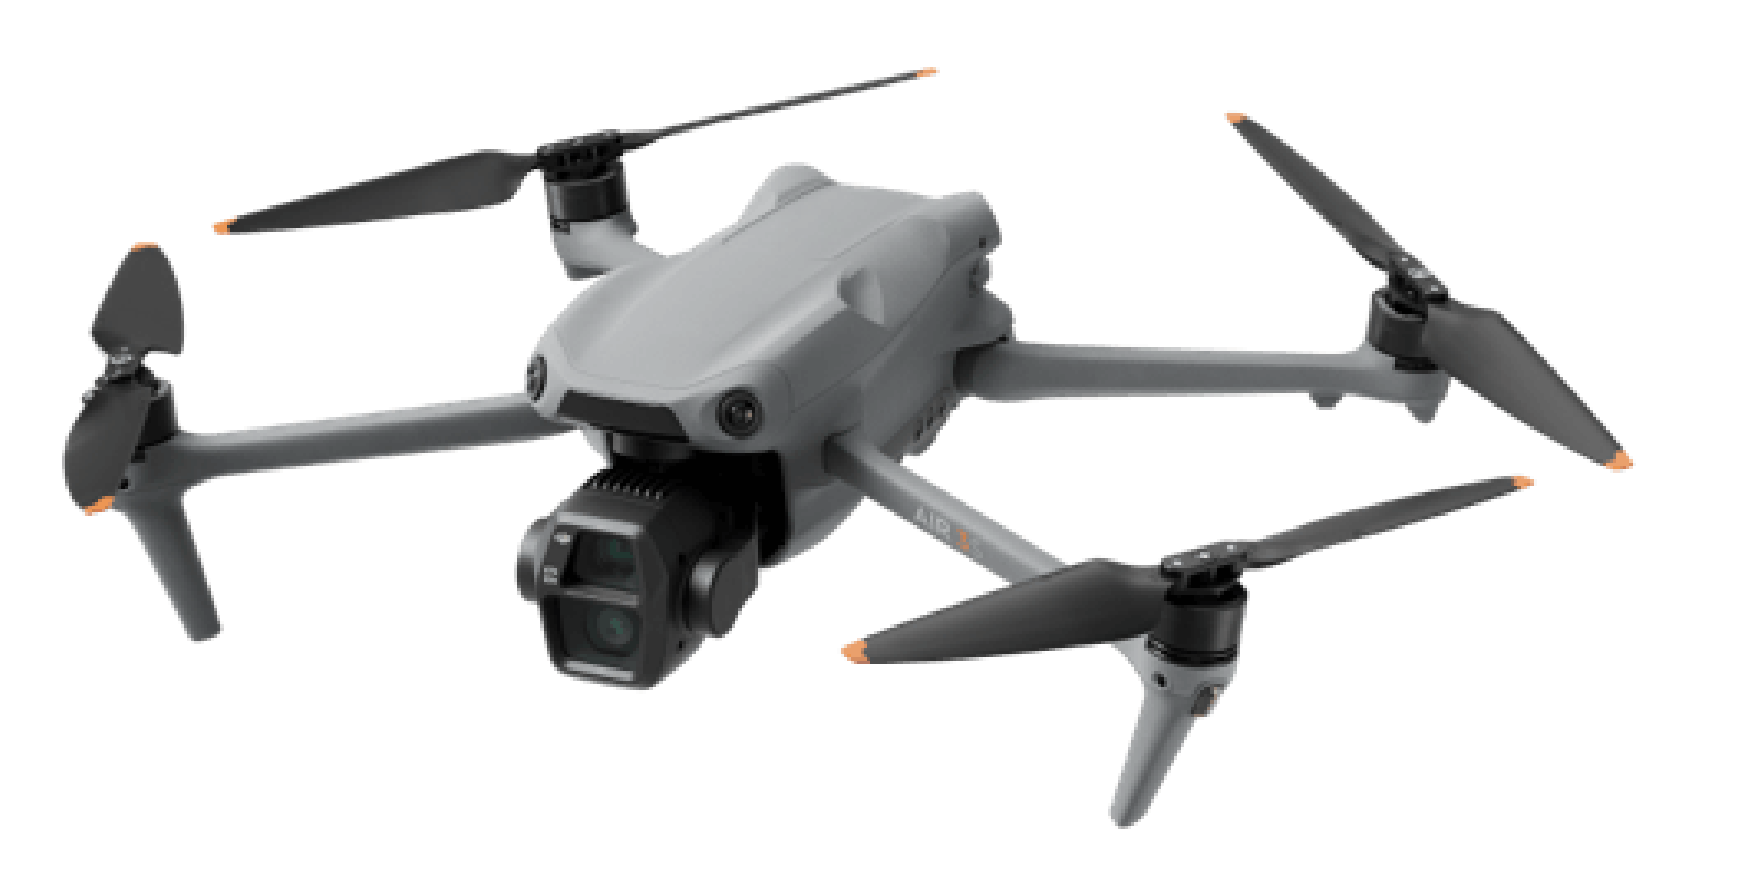
\includegraphics[width=0.45\textwidth]{imgs/MultiRotors.png}
    }
    \hfill
    \subfigure[Fixed-wing UAV]{
        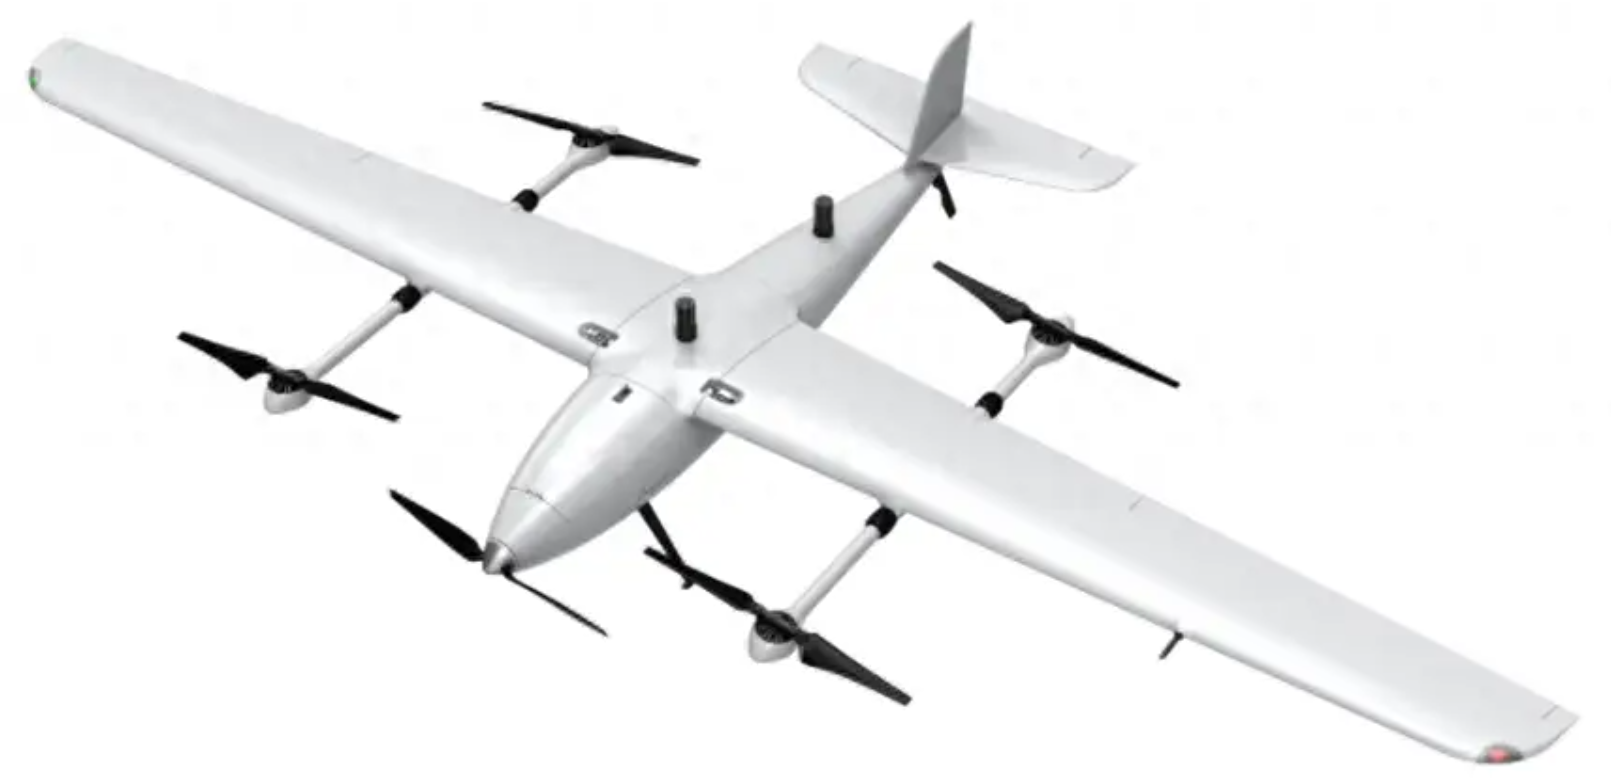
\includegraphics[width=0.45\textwidth]{imgs/FixWings.png}
    }
    \caption{The commonly types of UAV in civil engineering monitoring}
    \label{fig:UAVType}
\end{figure}

UAVs equipped with optical cameras primarily rely on mounted visible light cameras. By capturing a series of overlapping digital images from different positions and angles (typically nadir and planned oblique perspectives) \citep{guan2022review}, these images are processed using Structure from Motion (SfM) and Multi-View Stereo (MVS) algorithms. The SfM algorithm simultaneously computes the camera positions, poses, and a sparse 3D point cloud structure of the scene. Building upon this, the MVS algorithm utilizes geometric constraints and photometric consistency among multiple images to generate a dense 3D point cloud. Further processing can yield textured 3D mesh models, Digital Surface Models (DSM), and orthomosaic images. To ensure model quality, sufficient image overlap is required, with a typical recommendation of greater than 70\%-80\% for both forward and side overlap \citep{gonzalez2017unmanned,hu2023use}. This approach can be used for visual inspection, documentation and progress monitoring, 3D model generation and completion verification, and topographic surveying and earthwork volume calculation. However, the vertical (elevation) accuracy of optical measurements is typically lower than the horizontal accuracy. Furthermore, the processing results are suboptimal for surfaces lacking texture, that are excessively smooth, or exhibit uniform color, such as newly poured concrete, still water surfaces, or large areas of exposed wet clay \citep{wang2021multi}.

UAV-based LiDAR systems calculate target distance by measuring the round-trip time difference of laser pulses. By combining this with real-time UAV position and attitude information provided by high-precision Global Navigation Satellite Systems (GNSS) and Inertial Navigation Systems (INS)/Inertial Measurement Units (IMU), the 3D coordinates of the laser points are computed, generating a high-density point cloud. Unlike photogrammetry which is dependent on illumination, LiDAR is an active sensing technology and can acquire data independently \citep{yin2019individual}. LiDAR technology can directly and rapidly acquire high-precision, high-density 3D point cloud data of the excavation and its surrounding environment, enabling detailed geometric and topographic modeling. It can achieve earthwork volume calculation and high-precision deformation monitoring (with errors within 2mm) \citep{bao2025monitoring}. However, the cost and weight of its sensor system are typically higher than those of optical cameras, and data processing and analysis usually require specialized software and expertise, making it more complex than photogrammetry.

Air-based thermal imaging scanning detects infrared radiation emitted by object surfaces using sensors and converts it into visualized thermal images, where different colors or grayscale values represent different apparent temperatures. Thermal cameras mounted on UAVs typically operate in the long-wave infrared band. The temperature displayed in thermal images is the "apparent temperature", primarily used for seepage detection and water content variation mapping, thermal anomaly identification, and assisting in structural integrity evaluation \citep{wang2023removing,meng2022robust}. However, it measures the apparent surface temperature rather than internal temperature or direct physical parameters, and interpretation requires specialized knowledge and careful consideration of environmental factors. The spatial resolution is typically lower than that of optical cameras of the same class, and the cost is higher, making it less common in routine civil engineering construction monitoring \citep{zhang2024situ}.

\subsection{Ground Monitoring}
Excavation monitoring refers to the process of systematic measurement, analysis, and monitoring of key parameters—such as deformation, stress, and groundwater conditions—of the excavation support system, the foundation soil, and the surrounding environment (including adjacent buildings/structures, underground utilities, roads, etc.), using engineering surveying instruments and various sensors throughout the excavation and subsequent construction phases.

Excavation monitoring involves several key parameters, primarily including: Deformation Monitoring, Stress and Pressure Monitoring, Stability and Bearing Capacity Monitoring, and Groundwater Conditions.\citep{REN202330} Deformation Monitoring includes indicators such as: Ground Surface Settlement, Layered Settlement/Deep Soil Settlement, Lateral Displacement, Pit Bottom Heave/Rebound, Adjacent Building/Structure Deformation, and Adjacent Pipeline Deformation. Stress and Pressure Monitoring includes: Pore Water Pressure, Earth Pressure, Support/Anchor Axial Force/Stress, and Pile/Wall Stress/Strain. Stability and Bearing Capacity are often difficult to measure directly and are typically assessed indirectly through the monitoring of deformation and stress. Groundwater level monitoring is crucial for controlling water ingress into the pit, evaluating the effectiveness of dewatering systems, and analyzing the environmental impacts of drawdown outside the pit (such as inducing ground settlement and preventing soil erosion). This requires monitoring changes in both phreatic and piezometric heads inside and outside the excavation.

Before the widespread adoption of modern advanced monitoring technologies, traditional foundation monitoring methods constituted the primary means for ensuring safety in excavation engineering. These methods typically relied on manual on-site observations or semi-automated instrument readings, boasting a long history, mature techniques, and a wealth of accumulated engineering experience.\citep{LI20081519} Notably, even within the scope of traditional methods, there has been a trend towards electronic and automated evolution.\citep{CHENG2002375} For instance, the emergence of vibrating wire (VW) sensors (such as piezometers and strain gauges) and in-place inclinometers (IPIs) enabled remote automatic readings, overcoming some drawbacks of purely manual measurements and forming a bridge from traditional manual monitoring to modern automated monitoring.\citep{SIEBENMANN2015207} This article investigates the automated monitoring schemes, instrumentation, and parameters for the aforementioned common indicators, as presented in \autoref{tab:GroundMonitoring}. Notably, these advanced sensing technologies are not mutually exclusive but rather exhibit a trend towards integration and convergence. For instance, high-precision Fiber Bragg Grating (FBG) sensors can be deployed at critical locations, while Brillouin Optical Time/Frequency Domain Reflectometry/Analysis (BOTDR/A) is utilized to obtain overall deformation trends; Micro-Electro-Mechanical Systems (MEMS) sensors are integrated into Wireless Sensor Network (WSN) / Internet of Things (IoT) frameworks, enabling large-scale wireless monitoring; and fiber optic sensing can be employed for internal monitoring, complemented by remote sensing technologies for external environmental surveillance. This integration of multiple technologies allows for leveraging complementary strengths, thereby building more comprehensive and robust monitoring capabilities.

\begin{landscape}
\renewcommand{\arraystretch}{0.1}
\begin{longtable}{@{} >{\raggedright}p{3.5cm} >{\raggedright}p{4.5cm} >{\raggedright}p{5cm} >{\raggedright}p{4cm} >{\raggedright\arraybackslash}p{5.5cm} @{}}
    \caption{Analysis of Automated Monitoring Parameters for Excavation Engineering} \label{tab:GroundMonitoring} \\
    \toprule
    \textbf{Monitoring Parameter} & \textbf{Automated Method / Principle} & \textbf{Primary Automated Instrument} & \textbf{Key Measured Parameter} & \textbf{Remarks / Considerations} \\
    \midrule
    \endfirsthead
    
    \caption[]{Analysis of Automated Monitoring Parameters for Excavation Engineering (Continued)} \\
    \toprule
    \textbf{Monitoring Parameter} & \textbf{Automated Method / Principle} & \textbf{Primary Automated Instrument} & \textbf{Key Measured Parameter} & \textbf{Remarks / Considerations} \\
    \midrule
    \endhead
    
    % \midrule \multicolumn{5}{r}{{Continued on next page}} \\
    \multicolumn{5}{r}{{Continued on next page}} \\
    \endfoot
    
    \bottomrule
    \endlastfoot
    
    % --- Deformation Monitoring ---
    \multicolumn{5}{l}{\textbf{\textit{Deformation Monitoring}}} \\ \midrule
    Surface Settlement & Hydrostatic Leveling System (HLS); Automated Motorized Total Station (AMTS) & Automated HLS; Robotic Total Station + Prism & Vertical displacement (mm); 3D displacement (mm) & HLS: High precision, T/P sensitive. AMTS: 3D, line-of-sight/weather dependent. Stable benchmarks required. \\ 
    \midrule
    Layered / Deep Soil Settlement & Magnetic Extensometer (Automated probe); VW/FBG Multi-point Borehole Extensometer (MPBX); FBG Sensing Cable & Auto-probe + Magnetic Rings; VW/FBG MPBX; FBG Cable & Relative vertical displacement (mm) vs. datum & Requires borehole; Real-time (VW/FBG); Quasi-distributed (FBG); Datum stability critical. \\ 
    \midrule
    Lateral Displacement & Automated Inclinometer; AMTS; Shape Array (SAA) & Auto/MEMS Inclinometer; Robotic Total Station + Prism; SAA & Lateral displacement profile (mm); 3D displacement (mm); Deflection profile (mm) & Inclinometer: profile vs. depth. AMTS: surface points. SAA: continuous profile. Installation quality vital. \\ 
    \midrule
    Base Heave / Rebound & Extensometer (upward / deep datum); AMTS; VW/FBG Settlement Cell & Extensometer; Robotic Total Station + Prism; VW/FBG Settlement Cell & Vertical displacement (mm) & Access challenging during excavation; Requires stable reference/datum. \\ 
    \midrule
    Adjacent Structure Deformation & AMTS; HLS; Automated Crack Meter; Tiltmeter & Robotic Total Station + Prism; Automated HLS; VW/FBG/Resistive Crack Meter; MEMS/Electrolytic/VW/FBG Tilt Sensor & 3D displacement (mm); Differential settlement (mm); Crack width change (mm); Tilt (arcsec or mm/m) & Often multi-method approach; Baseline reading essential. \\ 
    \midrule
    Adjacent Pipeline Deformation & AMTS; Strain Gauges; Tiltmeters; SAA & Robotic Total Station + Prism/Target; VW/FBG Strain Gauge; Tilt Sensor; SAA & 3D displacement (mm); Strain ($\mu\epsilon$); Tilt (arcsec or mm/m); Deflection profile (mm) & Access often limited; Strain detects stress early; Utility owner coordination needed. \\ 
    \midrule
    
    % --- Stress and Pressure Monitoring ---
    \multicolumn{5}{l}{\textbf{\textit{Stress and Pressure Monitoring}}} \\ \midrule
    Pore Water Pressure & VW / Piezoresistive / FBG Sensing & VW / Piezoresistive / FBG Piezometer & Water Pressure (kPa or mH$_2$O) & Critical for effective stress \& stability; Filter saturation \& seal vital; Temp. correction (VW). \\ 
    \midrule
    Earth Pressure & VW / Strain Gauge / FBG Sensing & VW / Strain Gauge / FBG Earth Pressure Cell & Total Earth Pressure (kPa) & Measures total stress (needs PWP for effective stress); Proper installation/contact crucial. \\ 
    \midrule
    Support / Anchor Force / Stress & Strain Gauging; Hydraulic Load Cells & VW/Resistive/FBG Strain Gauge (welded/bonded); VW/FBG Rebar Meter/Axial Force Meter; Hydraulic Load Cell & Strain ($\mu\epsilon$) $\rightarrow$ Stress (MPa) / Force (kN); Direct Force (kN) & Temp. correction needed for strain gauges; Load cells give direct force; Calibration required. \\
    \midrule
    Pile / Wall Stress / Strain & Embedded / Surface Strain Gauging & VW Sister Bar; Embedment Strain Gauge (VW/FBG/Resistive); Surface Strain Gauge (VW/FBG/Resistive); FBG Sensing Cable & Strain ($\mu\epsilon$) $\rightarrow$ Stress (MPa) & Verifies design; Careful installation needed (embedded); Temp./creep/shrinkage effects. \\ 
    \midrule
    
    % --- Groundwater Monitoring ---
    \multicolumn{5}{l}{\textbf{\textit{Groundwater Monitoring}}} \\ \midrule
    Groundwater Level & Hydrostatic Pressure Sensing; Water Level Sensing & VW/Piezoresistive/FBG Piezometer/Water Level Sensor; Automated Water Level Meter & Water Level Elevation/Depth (m) & Monitors dewatering \& impact; Barometric compensation may be needed (vented sensors). \\ 
    \midrule
    % --- Stability ---
    \multicolumn{5}{l}{\textbf{\textit{Stability and Bearing Capacity}}} \\ \midrule
    Stability / Bearing Capacity & \multicolumn{3}{p{9cm}}{Indirectly assessed via analysis of deformation and stress/pressure monitoring data.} & Evaluation relies on trends, threshold comparison, and geotechnical analysis. \\
    
\end{longtable}
\renewcommand{\arraystretch}{1}
\end{landscape}

\subsection{Feasibility of SAG in Excavation Engineering}

Space-borne and air-borne monitoring technologies (key components of Space-Air-Ground, SAG, integrated systems) offer significant potential for excavation engineering. This is primarily due to their superior cost-effectiveness over traditional ground-based methods, their complementary technical characteristics, and the ability of surface monitoring data to, to some extent, reflect subsurface geotechnical mechanisms.

While ground-based monitoring currently predominates in excavation projects, the high cost of ground sensors hinders extensive deployment in large-scale developments. For instance, at China's Shanghai East Railway Station project (an excavation area exceeding 30 m), an automated inclinometer costs approximately \$138.17 USD per meter of measurement depth. For a 30m deep retaining wall, a single monitoring point for horizontal deformation would thus cost at least 4,145.19 USD (i.e., 30m × \$138.17/m). For this project, with 137 inclinometer points at an average depth of 35 m, a fully ground-based automated monitoring solution for this single indicator would cost approximately 663,000 USD. Air-borne and space-borne components of SAG monitoring systems effectively address coverage limitations: InSAR can readily monitor overall deformation of areas exceeding 100,000 m, and UAVs can survey a similar area in just 2-3 hours. The availability of these technologies enables combined application strategies based on differing technical characteristics, offering significant potential for optimizing precision, efficiency, and cost.

Due to their technical characteristics, space-borne and air-borne monitoring primarily target deformation. Key differences lie in measurement period, precision, and ease of use. Space-borne (e.g., InSAR) periods depend on satellite revisit times, while UAV monitoring can achieve hourly cycles for smaller projects. InSAR precision is linked to satellite data quality and cost, with high-precision ground-based InSAR requiring multiple units for full coverage \citep{rs11091029}. UAV survey precision, dependent on the mapping method, can reach millimeter-level with Ground Control Points (GCPs) \citep{MARTINEZCARRICONDO20181}. InSAR data processing requires specialized personnel and software, whereas UAV mapping and modeling demand minimal specific expertise. These characteristics, along with engineering experience, inform the selection of monitoring methods for excavations with different features, as summarized in \autoref{tab:monitoringSelection}.

\begin{table}[h]
    \centering
    \caption{Suggestions for selection in different engineering scenarios}
    \label{tab:monitoringSelection}
    \renewcommand{\arraystretch}{1.3}
    \begin{tabular}{p{6cm}p{4cm}p{6.5cm}}
        \toprule
        \textbf{Project Scale / Scenario} & \textbf{Recommended Monitoring Method} & \textbf{Description / Remarks} \\ 
        \midrule
        \textbf{<100m Small-scale Excavation (e.g., Municipal, Civil Defence)} & UAV Photogrammetry & Detailed modeling, accurate deformation capture, flexible deployment \\
        \textbf{100--300m Medium-scale Excavation (e.g., Rail Transit Station)} & UAV Photogrammetry + Local InSAR & Mainly UAV; InSAR for assessing far-field settlement trends \\
        \textbf{>300m Large-scale Excavation (e.g., CBD, Transport Hub)} & InSAR + UAV Dual Technology Integration & InSAR for wide coverage; identifying settlement troughs; UAV for detailed modeling to check structural displacement \\
        \textbf{Urban Agglomeration / Multiple Excavation Monitoring Context} & Mainly InSAR, UAV for auxiliary detailed inspection & InSAR provides continuous large-area background deformation; UAV for detailed review of key project sections \\
        \textbf{Emergency Incident / Rapid Deformation Response} & Rapid UAV flight preferred & Immediate on-site image + point cloud acquisition; rapid quantification of displacement or damage level \\
        \textbf{Long-term (>3 months) Evolving Settlement Assessment} & PS-InSAR preferred & Provides historical cumulative settlement trends, high temporal accuracy, suitable for soft ground monitoring \\
        \bottomrule
    \end{tabular}
\end{table}

Extensive research demonstrates correlations among various excavation monitoring indicators. For instance, positive correlations are observed between excavation depth, wall displacement, and surface settlement \citep{Ou2000DeepExcavation}; between wall displacement and both adjacent surface settlement \citep{Long2001DatabaseSupportedExcavations} and support axial forces \citep{Clough1989ConstructionInduced}. Groundwater level changes also correlate with deformations \citep{Finno2007ObservedPerformanceStruttedExcavation}, alongside continuous soft soil deformations \citep{Peck1969DeepExcavations} and abrupt data changes linked to construction sequences \citep{HE2020315}. If precise models describing these interrelationships can be developed, InSAR and UAV-based deformation monitoring could potentially infer parameters that are challenging for ground-based methods to monitor directly—such as pore water pressure, deep soil displacement, and support axial forces. This would significantly enhance monitoring efficiency and reduce the impact of automated monitoring on construction activities.

However, the discrete nature of monitoring data across different projects makes it difficult to establish universally applicable statistical relationships between indicators. Although researchers have identified typical correlation patterns in specific regions or similar soil conditions, these models often lack generalizability as they are not adequately linked to specific geotechnical properties, hindering widespread application \citep{HARAHAP2020103300}. If the interdependencies between various monitoring indicators can be accurately described, non-contact and remote sensing methods hold immense potential to revolutionize monitoring approaches in excavation engineering.


\section{Data Fusion and Analysis}

Multi-source data acquired from integrated SAG monitoring systems often exhibit characteristics such as heterogeneity (differing sources, formats, precision, frequencies), spatio-temporal inconsistency, uncertainty (noise, missing values, conflicts), and massiveness. Data from a single source or simple information superposition is often insufficient to comprehensively and accurately reflect the true state and potential risks of the excavations. Therefore, researching and applying advanced multi-source data fusion techniques to effectively integrate and analyze monitoring data from different sensors, times, and spatial locations is crucial for extracting more reliable, precise, and comprehensive information\citep{qin_chengzhi_recursive_2025}. Current mainstream data fusion methods include eight categories: Kalman filtering and its variants, Bayesian inference, Dempster-Shafer (D-S) evidence theory, neural networks, support vector machines (SVM), deep learning, tensor decomposition, and geospatial analysis.

\subsection{Data fusion framework}

In the monitoring and management of excavation engineering, effectively performing data fusion and analysis has become crucial when faced with large volumes of complex data from diverse sources. By integrating multi-source data from Space-Air-Ground (SAG) monitoring systems, we can obtain comprehensive and high-precision information on ground surface deformation and overall engineering status. However, this data often exhibits characteristics such as heterogeneity, spatio-temporal inconsistency, and noise issues, posing challenges for subsequent analysis and decision-making. Drawing from literature analysis, a broadly applicable advanced data analysis framework is presented, encompassing all stages from data acquisition, pre-processing, and data fusion to decision support. Through the fusion of multi-source data and an advanced analytics engine, this framework facilitates the transformation of complex raw data into actionable decision-making information, thereby enhancing the safety and construction efficiency of excavation projects. \autoref{fig:DataFusionFramework} illustrates the design concept of this integrated framework, showcasing the complete workflow from data acquisition to decision support, and detailing how different analytical methods and information products support engineering management decisions.

\begin{figure}[h]
    \centering 
    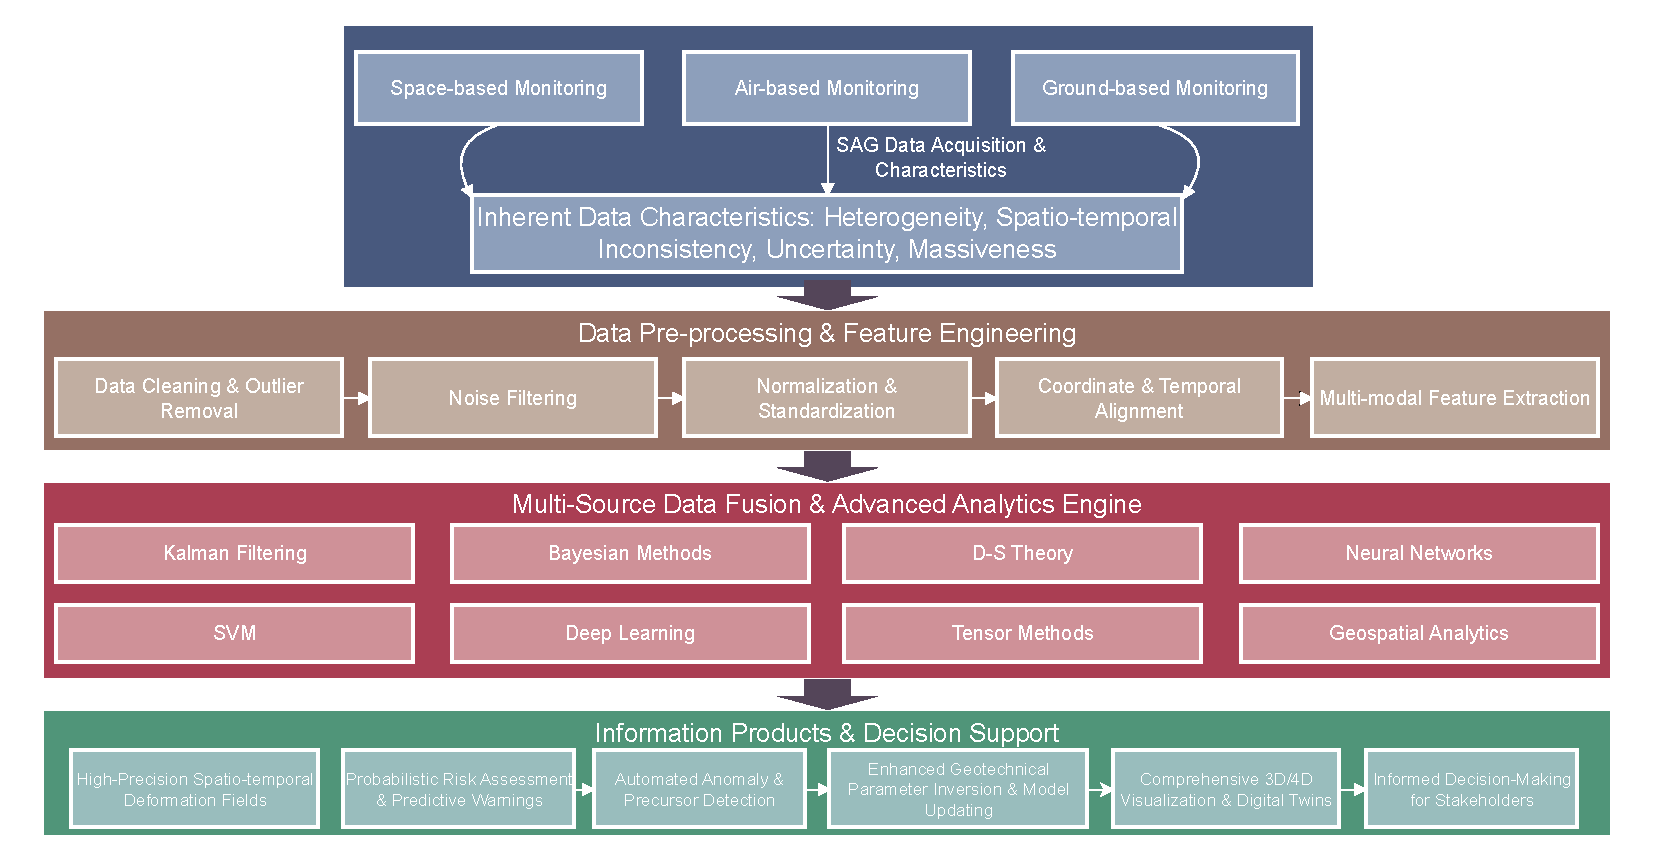
\includegraphics[width=\textwidth]{imgs/IntegratedAnalysis.pdf}
    \caption{A common multi-source data fusion and analysis framework}
    \label{fig:DataFusionFramework}
\end{figure}

\subsection{Kalman Filter}

The Kalman Filter (KF) is a powerful recursive Bayesian estimator for state estimation in noisy dynamic systems, utilizing a predict-correct cycle based on a dynamic model and measurements to optimize estimates \citep{khodarahmi_review_2023}. It predicts the current state from the previous estimate and model, then corrects it using current sensor data, rendering it the optimal linear filter. For non-linear problems common in soil mechanics or sensor models, variants like the Extended Kalman Filter (EKF), which employs Taylor series linearization \citep{3662552,Gelb1974}, and the Unscented Kalman Filter (UKF), which uses the Unscented Transform (UT) \citep{Julier1997}, are applied.

In intelligent excavations monitoring, KF and its variants primarily fuse multi-sensor time-series data to enhance deformation monitoring accuracy and reliability. Various sensors (e.g., GNSS, robotic total stations, inclinometers, hydrostatic levels) offer complementary strengths and weaknesses (e.g., GNSS provides absolute coordinates but suffers from multipath; total stations are precise but need line-of-sight). By defining a state vector representing deformation (e.g., 3D coordinates, velocity) and using a dynamic model (e.g., constant velocity/acceleration or more complex mechanical models), the KF predict-correct cycle integrates diverse sensor measurements to produce state estimates more accurate and reliable than those from single sensors \citep{SMYTH2007706}. For example, this fusion can reduce building settlement observation errors to below 24\% \citep{zhang2021processing}.

\subsection{Bayesian Inference}

Bayesian inference is a statistical method based on Bayes' theorem. Its core idea involves combining prior knowledge with observed evidence (data) to update the belief about a hypothesis or parameter, resulting in the posterior probability, as shown in \autoref{equ:BayesianInference}. This provides a powerful mathematical framework for reasoning and decision-making under uncertainty \citep{Gelman2013}. To apply Bayesian theory within complex event relationships, Bayesian networks were proposed to represent causal relationships and probabilistic dependencies in complex systems, supporting efficient probabilistic inference (such as prediction, diagnosis, and sensitivity analysis) \citep{Jensen2007}.

\begin{align}
    P(H|E)=\frac{P(E|H)\times P(H)}{P(E)}
    \label{equ:BayesianInference}
\end{align}

Where, $P(H \mid E)$ is the posterior probability, representing the probability of hypothesis H being true after observing evidence E. $P(E \mid H)$ is the likelihood, representing the probability of observing evidence E given that hypothesis H is true. $P(H)$ is the prior probability, representing the initial belief in hypothesis H being true before observing evidence E. $P(E)$ is the probability of the evidence, serving as a normalization constant.

Bayesian inference is crucial in excavations monitoring for managing uncertainty and integrating diverse information sources\citep{doi:10.1061/AJRUA6.RUENG-1363}. Key applications include:

\begin{itemize}
    \item \textbf{Multi-indicator Risk Assessment:} Bayesian networks (BNs) integrate multiple monitoring indicators (e.g., deformations, pressures) and influencing factors to probabilistically assess excavation risk levels. Real-time data updates risk probabilities via Bayesian inference, supporting warnings and decisions \citep{RiskAssessmentMethodology}.

    \item \textbf{Parameter Estimation \& Updating:} Prior knowledge regarding geotechnical parameters (from reports, experience) is formally combined with site-specific measurements (e.g., in-situ tests, monitoring data) via Bayesian updating to yield refined posterior parameter distributions \citep{WANG2016117}.

    \item \textbf{Heterogeneous Information Fusion:} Bayesian methods inherently fuse diverse information types, such as sensor data, model outputs, and expert judgments, at various integration levels (e.g., feature, decision) \citep{CAO2016107}.

    \item \textbf{Uncertainty Quantification \& Propagation:} Represents and propagates uncertainties associated with parameters, models, and data using probability distributions. This yields probabilistic results (e.g., distributions, confidence intervals) vital for reliability and risk analysis, going beyond point estimates \citep{WANG2025108098}.
\end{itemize}

\subsection{Dempster-Shafer Theory}

Dempster-Shafer (D-S) evidence theory, originated by Dempster and developed by Shafer, provides a general framework for reasoning under uncertainty. Often considered a generalization of Bayesian theory, it particularly excels at handling uncertain, imprecise, or conflicting information sources. Key concepts include the frame of discernment ($\Theta$), basic probability assignment (BPA or mass function, $m$), belief (Bel), and plausibility (Pl) functions. Unlike Bayesian probability, D-S theory does not require prior probabilities and explicitly represents ignorance by assigning belief mass to sets of hypotheses rather than only singletons.
D-S theory offers distinct advantages for fusing potentially conflicting or uncertain information in excavations monitoring, including:

\begin{enumerate}
    \item \textbf{Dynamic Risk Assessment \& Multi-Source Fusion:} D-S theory can fuse potentially conflicting real-time data from various sensors monitoring excavations status. Each sensor acts as an evidence source, providing belief mass regarding specific states (e.g., stability or risk levels), enabling dynamic risk assessment \citep{ABELLAN2021114987}.

    \item \textbf{Safety Assessment with Heterogeneous Data:} It allows fusing quantitative monitoring data with qualitative information (e.g., geological reports, expert opinions), potentially combined with methods like fuzzy sets. Both data types are converted to basic belief assignments (BBAs) and fused using Dempster's rule to yield a comprehensive safety assessment, explicitly quantifying belief and uncertainty across different safety states \citep{wu_collapse_2024}.

    \item \textbf{Specific Risk Evaluation (e.g., Water Inrush):} D-S models can assess specific risks like water inrush by treating contributing factors (or their indicators) as evidence sources. Belief masses assigned to different risk level hypotheses are fused to provide an overall risk judgment, effectively handling incomplete or conflicting evidence \citep{buildings14093022}.
\end{enumerate}

Key challenges in applying D-S theory include determining appropriate BBAs, which often relies on other models or expert judgment, potentially introducing subjectivity \citep{AMultiSourceIntelligent}. Selecting suitable conflict handling strategies and measuring evidence reliability remain active research areas \citep{ZHAO2022109075}. Furthermore, the computational complexity of Dempster's rule grows exponentially with the size of the frame of discernment, potentially limiting application to complex problems with numerous states \citep{LI2021103948}.

\subsection{Neural Networks}

Neural Networks (NNs), particularly Backpropagation Neural Networks (BPNN) and Long Short-Term Memory (LSTM) networks, are powerful data-driven models excelling in processing complex non-linear relationships and time-series data for classification and prediction. They find widespread application in excavations deformation prediction and intelligent monitoring \citep{WU2023184, YANG2024, XIE2022101313}. Commonly applied models include:

\begin{enumerate}
    \item \textbf{Backpropagation Neural Networks (BPNN):} Standard feedforward NNs (often termed ANNs) that map input features (e.g., geological/geometric parameters, current monitoring data) to outputs (e.g., deformation, stability factors). Performance can be enhanced using optimization algorithms (e.g., GA-BPNN) \citep{LU2023139241}.

    \item \textbf{Recurrent Neural Networks (RNNs):} Especially LSTMs and GRUs, these are designed for sequential data, ideal for analyzing and predicting excavations monitoring time-series (e.g., future displacements from historical data) by capturing temporal dependencies. Bidirectional variants (e.g., BiLSTM) are also common \citep{LI2023105243}.

    \item \textbf{Hybrid Neural Networks:} Combine different architectures (e.g., CNN-LSTM) or techniques (e.g., Wavelet transforms, Attention mechanisms) to leverage strengths, such as using Convolutional Neural Networks (CNNs) for feature extraction from spatial/temporal data before LSTM processing \citep{zhao2025early}.

    \item \textbf{Radial Basis Function Networks (RBFN):} Another feedforward network type used for function approximation and predicting excavation-induced responses, sometimes offering faster training than BPNNs \citep{zhou_performance_2021}.
\end{enumerate}

\subsection{Support Vector Machine}

Support Vector Machines (SVM) are powerful supervised learning algorithms for classification and regression, particularly effective with high-dimensional data and small sample sizes \citep{Murphy2022Intro}. The core principle involves finding an optimal hyperplane that maximizes the margin between different data classes, defined by the nearest data points (support vectors), which promotes good generalization. For non-linear data, the kernel trick implicitly maps data to higher-dimensional spaces for linear separation, utilizing common kernels like Linear, Polynomial, Radial Basis Function (RBF), and Sigmoid. SVMs adapted for regression are termed Support Vector Regression (SVR). In intelligent excavations monitoring, SVMs are primarily utilized for stability classification or risk prediction based on features derived from multi-source monitoring data. Applications include:

\begin{enumerate}
    \item \textbf{Stability Classification:} Define pit stability states (e.g., 'Stable', 'Unstable', 'Alert', 'Danger'). Features derived from fused multi-sensor data (e.g., maximum displacement, deformation rates, stress ratios, water pressure changes) are used as input to train SVM classifiers for determining the current stability status \citep{LI20231019}.

    \item \textbf{Risk Level Prediction:} Similarly, SVM models can be trained using fused monitoring features and influencing factors (e.g., geological conditions, excavation depth, support parameters) to predict the overall risk level associated with the excavation \citep{PAN2024109578}.

    \item \textbf{Integration with Other Methods:} SVMs can function within broader information fusion frameworks. For example, an SVM's preliminary risk classification could serve as input evidence for D-S theory or Bayesian networks. Alternatively, SVMs can aid in feature selection, identifying the most influential monitoring indicators for stability \citep{WU2024105516}.
\end{enumerate}

\subsection{Deep Learning}

Deep Learning (DL), a subfield of machine learning, employs deep neural networks (DNNs) with multiple layers to automatically learn hierarchical features and recognize patterns from raw data. This capability, eliminating the need for manual feature engineering required by traditional methods, has led to breakthroughs in image analysis, natural language processing, and time-series prediction, showing significant potential for civil engineering monitoring. DL excels at handling high-dimensional, complex, and unstructured data common in monitoring. Convolutional Neural Networks (CNNs), a prominent type of DNN, are frequently used in excavations engineering for image and video analysis tasks, including:

\begin{enumerate}
    \item \textbf{Crack Detection and Quantification:} CNN architectures (e.g., U-Net, FCN, Mask R-CNN) automate pixel-level detection, segmentation, and localization of cracks on structural surfaces (retaining walls, supports, adjacent buildings) from images or video. This allows for precise quantification and monitoring of crack evolution using temporal image sequences \citep{https://doi.org/10.1002/stc.2981}.

    \item \textbf{Site Safety and Environmental Monitoring:} Object detection CNNs (e.g., YOLO, SSD, Faster R-CNN) analyze video streams to automatically identify hazards such as improper PPE usage, zone intrusion, unsafe equipment proximity, visual signs of instability, or water ponding. Multi-camera setups enhance coverage, while temporal architectures (e.g., 3D CNN, CNN+RNN) allow analysis of dynamic events \citep{LIU2022104302}.

    \item \textbf{Vision-Based Deformation Monitoring Assistance:} CNNs can enhance vision-based deformation monitoring by improving tasks like target recognition or extracting relevant displacement features from images/videos. This CNN-derived visual information can then be fused with data from traditional sensors (e.g., inclinometers, settlement gauges) using techniques like Kalman filtering or Bayesian inference for more robust state estimation \citep{SHEN2023100442}.

    \item \textbf{3D Reconstruction and Reality Modeling:} Techniques like Structure from Motion (SfM) and Multi-View Stereo (MVS), often utilizing UAV imagery, generate high-fidelity 3D models of the pit and surroundings by fusing numerous 2D images. CNNs can contribute by enhancing key steps like feature matching, depth estimation, or adding semantic understanding to the reconstructed models \citep{WU2021103706, rs14205187}.
\end{enumerate}

Transformer models, initially achieving great success in natural language processing through their core self-attention mechanism, effectively capture long-range dependencies in sequential data and offer parallel computation benefits \citep{Vaswani2017Attention}. They are increasingly applied to time-series forecasting, potentially outperforming traditional Recurrent Neural Networks (RNNs) like Long Short-Term Memory (LSTM), particularly for the long sequences (spanning months or years) typical of excavations deformation monitoring data. Such data are often influenced by multiple long- and short-term factors (geological, hydrological, constructional, environmental). The self-attention mechanism allows Transformers to potentially fuse long time-series data from multiple sensors (e.g., displacement, stress, water level, rainfall) more effectively, capturing complex temporal patterns and cross-variable dependencies to achieve more accurate long-term deformation predictions \citep{Nie2023PatchTST}. For instance, the LE-Transformer model fused Interferometric Synthetic Aperture Radar (InSAR) time-series data with multiple influencing factors (e.g., rainfall, subway construction, temperature, hydrogeology) for deformation prediction, achieving a Mean Absolute Percentage Error (MAPE) of 2.5\% \citep{rs17061106}.

Furthermore, hybrid deep learning approaches combining different models are explored to enhance performance. For example, integrating Convolutional Neural Networks (CNNs) with LSTMs leverages the spatial feature extraction capabilities of CNNs and the temporal sequence modeling strengths of LSTMs. This hybrid CNN-LSTM architecture can effectively fuse spatio-temporal monitoring data (e.g., incorporating spatial patterns of surface settlement or retaining wall deflections over time) and has been successfully applied to predict surface settlement in excavations \citep{zhao_spatiotemporal_2021, WANG2024105733}.

\subsection{Tensor Decomposition}

Traditional matrix-based analysis struggles with the complex structures and latent correlations within high-dimensional, multi-aspect monitoring data (e.g., involving time, space, sensor types). Tensor Decomposition (or Factorization) offers key techniques to extract latent structures, reduce dimensionality, and discover hidden patterns within such higher-order tensor data \citep{7891546}. Representing, for instance, excavations monitoring data as a 4th-order tensor $\chi$ (e.g., dimensions: location, time, sensor type, parameter value) preserves inherent multi-way structural information often lost during matricization \citep{adarkwa2015tensor}. Common tensor decomposition methods used in multi-source data fusion include \citep{SALEHI2023106659}:

\begin{enumerate}
    \item \textbf{CANDECOMP/PARAFAC (CP):} Decomposes a tensor into a sum of rank-1 tensors (outer products of factor vectors). It identifies latent factors capturing the main data variations, useful for data compression, identifying dominant modes (e.g., peak times, structural modes), and detecting anomalies or pattern changes reflecting collective behavior or construction impacts.

    \item \textbf{Tucker Decomposition:} Represents a tensor using a core tensor (for mode interactions) and factor matrices (principal components per dimension). Flexible ranks suit multi-modal data analysis, such as fusing sensor data for structural mode identification or analyzing temporal data for change detection. Non-uniqueness can be addressed with constraints/regularization.

    \item \textbf{Tensor Train (TT):} Decomposes a high-order tensor into a chain-like product of smaller (typically 3rd-order) tensors (TT-cores), linked by TT-ranks. This tensor network representation significantly reduces storage and computational complexity, especially for very high-order tensors (N>4), scaling linearly rather than exponentially. Suitable for compression, online updating, long-term prediction, and modeling multi-source coupling in large-scale monitoring systems.

    \item \textbf{Tensor Ring (TR):} Extends the TT decomposition by connecting the first and last TT-cores, forming a ring structure. This removes boundary constraints and enhances representational capacity, particularly for data with periodic or symmetric properties. Potential applications include modeling cyclical construction processes or compressing spatio-temporal data like image/video tensors.
\end{enumerate}

\subsection{Geospatial Analysis Methods}

Excavations monitoring data possess inherent spatio-temporal attributes, with readings taken at specific locations over time. Geospatial analysis methods, particularly Geographic Information Systems (GIS) and Spatio-temporal Data Mining (STDM), provide powerful tools for fusing, analyzing, and visualizing these data. Key research directions include spatial interpolation combined with GIS overlay analysis, and spatio-temporal data mining \citep{WANG201941}.

Spatial interpolation techniques estimate values at unsampled locations based on discrete monitoring points (e.g., settlement, displacement) to generate continuous spatial distribution maps, such as deformation fields or contour plots. Kriging is a common geostatistical method used for this, considering both distance and spatial autocorrelation between sample points \citep{TERRANOVA2015105}. Applying Kriging to excavations monitoring data allows for the creation of continuous settlement or displacement maps, facilitating the identification of deformation concentration zones, high-gradient areas, and overall patterns. These interpolated maps can then be visually overlaid with other relevant layers within a GIS (e.g., geological strata, adjacent structures) to analyze spatial relationships and potential impacts \citep{Spinetti18082019}.

Spatio-temporal Data Mining (STDM) focuses on discovering non-trivial, hidden patterns and knowledge from large datasets incorporating both space and time. STDM considers spatial and temporal autocorrelation as well as their interactions, employing techniques like spatio-temporal clustering, association rule mining, outlier detection, and prediction. Applying STDM to fused multi-source monitoring data can help identify deformation hotspots, reveal spatio-temporal correlations, and detect abnormal patterns or events \citep{FESTA20221}.

\section{Representative Case Studies}

Typical global case studies of integrated SAG monitoring for excavations, as summarized in \autoref{tab:excavation_monitoring}, reveal that most projects combine two methods due to site constraints, usually pairing core ground-based monitoring with either space-based or air-based techniques. In these integrated systems, fundamental ground-based monitoring for essential structural safety data is complemented by space-based techniques for large-area settlement observation and data validation, and by air-based methods for site-wide photogrammetry to capture detailed surface features and track deformation. This combined approach effectively monitors large-scale settlement and key surrounding structures, highlighting the key advantage of SAG systems: the ability to synergistically balance coverage, cost, and precision by combining wide-area space/air monitoring with high-accuracy local ground sensors. Three typical monitoring cases of excavation projects will be briefly analyzed as following sections.

\begin{landscape}
\begin{table}[htbp]
  \centering
  \caption{Cases of integrated monitoring of SAG for excavation projects}
  \label{tab:excavation_monitoring}
  \begin{tabular}{p{4cm}p{5cm}p{5.5cm}p{5cm}p{5cm}p{5cm}}
    \toprule
    Case study (location, type) &
    SAG components (aerial / space-based / ground-based) &
    Integration methods / platforms &
    Main monitoring objectives &
    Key findings / results &
    Main challenges / limitations \\
    \midrule
    Deep excavation in Beijing \citep{buildings15030366} &
    Ground-based (AMTS, cameras, anchor load cells) &
    Digital twin (ABAQUS + GA back analysis), 5G, cloud database &
    Risk simulation, prediction and control; real-time / predictive early warning &
    DT model updated with prediction error $<10\%$; more timely and accurate early warning &
    On-site information integration; data-transmission capacity; influence of observation errors; limitations on internal-force output \\
    \midrule
    Subway station pit in Shenzhen \citep{AnIntegratedIntelligent} &
    Aerial (UAV), ground-based (MEMS inclinometer, FOS-BOFDA, MV), subsurface (BIM geological model) &
    Digital twin platform, multi-source sensing fusion &
    Full-lifecycle intelligent monitoring and management; real-time high-precision monitoring; parameter prediction &
    Verified feasibility of multi-source sensing integration; GA-BP prediction effective; DT platform achieves comprehensive management &
    Complexity of integrating multiple advanced technologies \\
    \midrule
    Gesaer gold-mine subsidence \citep{chen_mining_2025} &
    Space-based (InSAR, GNSS verification), aerial (UAV) &
    IoT framework, UAV / InSAR threshold-segmentation fusion, GA-BP prediction &
    Analysis of mine-area subsidence deformation; addressing line-of-sight (LOS) deformation and direction inconsistency &
    Fusion solves InSAR decoherence and UAV edge-precision issues; GA-BP prediction effective; reveals subsidence patterns &
    InSAR decoherence in large-deformation areas; low UAV precision for small deformations; insufficient UAV data for prediction \\
    \midrule
    Excavation alongside Toronto railway \citep{GeoWeekNewsMonirDT} &
    Aerial (UAV + iTwin Capture), ground-based (AMTS + prisms, IoT sensors) &
    Bentley iTwin IoT platform (DT), OpenGround integration &
    Monitoring of railway displacement and excavation site; ensuring railway-operation safety &
    40\% improvement in operational efficiency; 3000 evaluation man-hours saved; project duration reduced by 6 months; \$1 million scope-cost reduction &
    AMTS line-of-sight affected by slope; strict monitoring requirements \\
    \midrule
    Glòries Square tunnel dewatering \citep{BOTEYIBASSOLS2021106041,SERRANOJUAN20171} &
    Space-borne (D-InSAR: Sentinel-1), ground-based (levelling surveys, piezometers) &
    Complementary use of D-InSAR and levelling data; analysis with hydrogeological data &
    Monitoring of ground deformation caused by dewatering; understanding deformation phenomena &
    D-InSAR reveals spatio-temporal distribution and cause of deformation; levelling provides more accurate quantification &
    (Not explicitly mentioned) \\
    \midrule
    Naples subway tunnel \citep{rs15102555} &
    Space-borne (MT-InSAR: COSMO-SkyMed), ground-based (precision levelling points) &
    Comparison of InSAR and levelling; Gaussian-curve fitting for settlement data to estimate volume loss &
    Monitoring of vertical displacement caused by tunnel excavation; evaluation of volume loss &
    Good agreement between InSAR and levelling results; volume loss within expected range (0.5-1 \%) &
    MT-InSAR real-time capability limited by revisit period and phase ambiguity \\
    \midrule
    London Crossrail project \citep{marti2017use} &
    Space-borne (InSAR: TerraSAR-X), ground-based (levelling, prisms) &
    InSAR as a supplement to traditional ground-based monitoring &
    Construction control; protection of third-party assets; post-construction settlement monitoring &
    InSAR effective for post-construction monitoring and baseline acquisition; more cost-effective than maintaining automated-prism system &
    X-band sensitivity limited for rapid / large deformations; phase-unwrapping errors \\
    \bottomrule
  \end{tabular}
\end{table}
\end{landscape}

\subsection{Shenzhen Subway Station Project}

The Waterlands Resort East Station in Shenzhen is a large underground transfer station ($543.7\;\mathrm{m}$ long, $19.7\;\mathrm{m}$ wide, excavation depth $17.5$-$18.5\;\mathrm{m}$) constructed by open‐cut method with diaphragm‐wall support. The dense urban context, soft-soil conditions and long excavation length created a demanding monitoring scenario requiring millimetric accuracy and real-time feedback.

Hong et al. proposed a “transparent-geology-multi-source perception-deep-learning-digital-twin” workflow, integrating: \emph{Space/Ground.} BOFDA distributed optical fibres embedded in the diaphragm walls ($0.05\;\mathrm{m}$ spatial resolution, strain baseline $\sim\!5100\,\mu\varepsilon$) for continuous strain/temperature profiles. \emph{Air.} UAV photogrammetry for 3-D surface morphology and progress audits; machine-vision (MV) cameras for non-contact settlement tracking (MV-total-station residuals $<\!1\;\mathrm{mm}$). \emph{Ground.} Wireless MEMS inclinometers (tilt range $0$-$60^{\circ}$, $R^{2}=0.99$ in calibration) and conventional sensors (water-levels, total stations) to capture support deformation, axial force and pore pressure.

These data streams were pushed via IoT gateways to a cloud BIM-WebGIS platform, ensuring coordinate harmonisation and automated alarm logic. Four neural-network models (BP, GA-BP, NARX, Elman) were trained on one-year monitoring data.  GA-BP yielded the lowest RMSE for axial force, settlement and horizontal displacement prediction, providing a reliable $T\!+\!3$-day early-warning tool.  Model back-testing is embedded in the dashboard, allowing engineers to switch algorithms on demand.
A mobile DT App (Unity3D + ARCore) synchronises the BIM model, real-time sensor feeds and ML forecasts.  Field staff can disassemble the 3-D model, query any component’s live data and roam the excavation in augmented reality to visualise risk hotspots.  The same platform will host operation \& maintenance (O\&M) data after station commissioning, realising full-lifecycle monitoring.

The result shows that multi-source fusion reduced single-sensor bias and provided redundant observables; MEMS-BOFDA correlations kept wall-top displacement prediction within $\pm2\;\mathrm{mm}$ at peak excavation. Lifecycle integration (survey $\rightarrow$ BIM $\rightarrow$ DT) shortened design-construction information loops and enabled proactive decision making. Challenges remain in long-term sensor stability and high-frequency data storage ($>5\;\mathrm{GB\,day^{-1}}$). The authors adopted edge pre-filtering and layered Kalman/Bayesian fusion to manage bandwidth and consistency issues.

\subsection{Naples Subway Tunnel}

To connect Capodichino Airport with the city centre, two parallel 1 km TBM tunnels (7 m diameter, axis depth 40 m → 10 m) were bored between the future Capodichino and Poggioreale stations on Naples Metro Line 1. The alignment passes beneath densely built terrain and the historic Poggioreale cemetery, requiring millimetric deformation control.
The study adopted a purely \emph{Space-Ground} strategy centred on Multi-Temporal InSAR (MT-InSAR). A stack of 237 COSMO-SkyMed X-band Stripmap images (3 m resolution, ascending geometry, 7 Mar 2018 - 29 Jan 2022) was processed with the persistent-scatterer module of SARPROZ. About 20 000 coherent targets ($\approx$30 000 PS km\textsuperscript{-2}) were extracted over the area of interest, giving full-coverage settlement information at millimetric precision.

\emph{First tunnel}: MT-InSAR settlements were fitted with a Gaussian trough to derive volume-loss $V_\mathrm{L}$ and inflection distance $i_x$ (K-ratio). Best-fit $V_\mathrm{L}$ ranged 0.5 - 1.0 \%—typical for EPB TBM in soft rock. \emph{Second tunnel}: the same $V_\mathrm{L}$ and $i_x$ were imposed and the two troughs superposed to predict the total settlement profile. MT-InSAR captured a clear subsidence bowl centred on the first (eastern) tunnel and, after September 2021, a twin trough after the second drive. Predicted and observed settlements agreed in both shape and magnitude (max 9-13 mm), validating the use of MT-InSAR-derived $V_\mathrm{L}$ for forward prediction. Continuous spaceborne coverage offered a dense, non-intrusive complement to sparse ground instruments, suitable for post-processing-based risk assessment of hundreds of surface structures.

The satellite workflow delivered city-scale deformation maps without site access, but two constraints remain: (i) 16-day CSK revisit hinders true real-time alarms, and (ii) phase ambiguity can mask rapid displacements above $\lambda/4$ between acquisitions. Hybrid SAG schemes incorporating UAV or GNSS could mitigate these gaps in future projects. The case confirms that \emph{wide-area MT-InSAR + selective ground sensors} is a cost-effective recipe for urban twin-tunnel monitoring. Early extraction of $V_\mathrm{L}$ from the first drive provides reliable input for predictive control of subsequent excavations, demonstrating a transferable strategy for other metro extensions.

\subsection{London Crossrail Project}

Crossrail’s 21 km twin-bore tunnels run beneath Central London, intersecting a dense legacy of third-party assets.  During the post-excavation phase the project team trialled satellite interferometry to replace or supplement thousands of automated‐prism and manual-levelling points distributed along the alignment.  The case study was collated in the Crossrail \textit{Learning Legacy}. The \emph{space-ground} layers were activated in this phase: \emph{Space.} Two TerraSAR-X X-band satellites in constellation, StripMap mode (30 km × 50 km swath, 3 m pixels), 11-day revisit. Persistent-scatterer interferometry (PSI) processing yielded $\sim$20 000 stable scatterers over the central tunnelled zone. \emph{Ground.}  Legacy UCIMS data sets—automated total-station prisms, manual levelling and track gauges—served as truth points for calibration and phase-offset correction.\emph{Integration.}  Quarterly PSI point clouds were delivered as CSV and loaded into \textit{Geoscope 7} and ArcGIS; planned integration with the UCIMS geodatabase was under development.

This monitoring initiative had three primary objectives: establishing a wide-area baseline before the completion of heavy civil works, confirming post-construction settlement remained under 2 mm yr$^{-1}$ for asset handover, and lowering the long-term maintenance cost of dense ground-instrument arrays.
The results confirmed the value of the approach. Financially, annual PSI data processing for the 50 km $\times$ 30 km corridor was an order of magnitude cheaper than maintaining the full prism network. The method's performance was validated at key sites like Whitechapel and Farringdon, where PSI-derived settlement rates (e.g., $\approx$ 9 mm yr$^{-1}$) correlated well with prism data. Furthermore, the technique provided crucial regional context by revealing a city-wide seasonal heave-settlement cycle, helping to distinguish it from construction-induced impacts.
However, key limitations were noted, including a motion detection cap of ±15 mm between images due to the X-band wavelength, with larger movements causing phase-unwrapping errors. The 11-day revisit period is suitable for slow post-construction monitoring but too infrequent for tracking rapid movements during active construction (e.g., TBM drives). Additionally, data coverage is sparse over vegetation and water due to poor backscatter.
  
\section{Conclusion}

\subsection{Challenges and Limitations}

\subsection{Challenges and Limitations}\label{sec:challenges}

Despite the demonstrable advantages of Space--Air--Ground (SAG) integrated monitoring, several bottlenecks must be overcome before the technique can reach routine, real-time deployment in large-scale excavations. These challenges fall into two main categories: sensor technology and engineering management. Within sensor technology, the primary issues include:

\begin{itemize}
  \item \textbf{InSAR} suffers from atmospheric-delay errors, temporal/spatial decorrelation and wavelength-limited phase ambiguity, which impede the detection of rapid displacements and demand complex time-series processing.
  \item \textbf{UAV photogrammetry/LiDAR} is weather-dependent; its vertical accuracy hinges on dense Ground Control Points, and image-matching quality deteriorates on low-texture surfaces.
  \item \textbf{GNSS} provides centimetre-level precision only when short baselines or dense CORS services are available; multipath interference, antenna quality and lengthy PPP convergence restrict in-field usability.
\end{itemize}

Within engineering management technology:

\begin{enumerate}
    \item \textbf{Economic and logistical issues:} High-precision ground instruments remain costly. At Shanghai East Railway Station, an automated inclinometer array alone would exceed USD 0.66 million, preventing dense coverage in mega-projects.
    \item \textbf{Data fusion and management:} Heterogeneous, asynchronous streams can exceed 5 GB day$^{-1}$ in long-term campaigns, challenging bandwidth, storage and computation. Classical fusion frameworks (Kalman, Bayesian, D-S) require careful evidence weighting, and D-S complexity escalates exponentially with the number of hypotheses.
    \item \textbf{Model transferability:} Monitoring datasets are highly project-specific and discretely sampled. Correlation models calibrated on one site often lack generalisability to different geology or construction sequences, hampering the development of universal predictive tools.
    \item \textbf{Regulatory fragmentation:} While some Chinese municipal codes embed SAG concepts, many jurisdictions still rely on traditional ground-centric standards, leading to heterogeneous data-quality requirements and acceptance criteria across regions.
    \item \textbf{Operational reliability:} Long-term field deployment faces sensor drift, power-supply issues and construction-related damage. Maintaining calibration and data continuity over multi-year projects therefore remains non-trivial.
\end{enumerate}

In summary, current SAG monitoring systems deliver unprecedented spatial coverage and multi-scale insights, yet their full potential is curtailed by sensor physics, economic constraints, big-data management and the absence of harmonised standards. Addressing these limitations will be essential for the next generation of intelligent, risk-responsive excavation monitoring platforms.

\subsection{Discussion and Future Outlook}

This review confirms that SAG integrated monitoring has matured from an exploratory concept into a technically viable paradigm for large-scale excavation projects. Publication statistics show an exponential rise in SAG-related studies since 2010, with UAV- and InSAR-borne solutions driving the growth curve, while ground and GNSS techniques remain steady mainstays of data validation.  Case analyses further demonstrate that dual- or tri-modal configurations consistently outperform single-sensor schemes by balancing wide-area coverage, local precision and cost efficiency.  Nonetheless, the review also reveals persistent fragmentation in standards and data management practices across jurisdictions, hindering large-scale interoperability.

Combining satellite, UAV and ground sensors delivers multi-scale deformation insight, supports rapid cross-checks and feeds digital-twin risk models that attain forecasting errors below 10\% in complex urban pits. Yet, our synthesis shows that InSAR and UAV data still serve mainly as \emph{surface} proxies, with limited linkage to subsurface stress paths or pore-pressure evolution.  Ground instrumentation therefore remains indispensable for causal diagnosis.  Bridging this surface-subsurface divide will require physics-guided learning that embeds constitutive constraints into data‐driven fusion pipelines.

Four technology trends are poised to reshape SAG monitoring in the future:

\begin{enumerate}
    \item \textbf{AI-enhanced fusion.}  Deep generative models, graph neural networks and tensor decomposition are already moving from proof-of-concept to field trials for uncertainty-aware fusion of asynchronous, heterogeneous streams.  Their deployment promises centimetre-level deformation fields at daily cadence.
    \item \textbf{Ubiquitous low-cost sensing.}  Mass-produced MEMS inclinometers, microwave links and smartphone GNSS chips can form dense ground networks to complement wide-area satellites, lowering whole-life monitoring costs by an order of magnitude.
    \item \textbf{Edge-cloud analytics.}  Hybrid architectures that run first-pass anomaly detection on site (edge) and deeper inversion in the cloud will shorten decision latency from hours to minutes, vital for active risk mitigation.
    \item \textbf{Next-gen satellite constellations and UAV swarms.}  Sub-daily C-/L-band SAR constellations and autonomous multirotor swarms will improve spatio-temporal resolution, enabling near-real-time digital twins for construction control.
\end{enumerate}

To unlock the full potential of SAG monitoring, the following priorities are recommended:

\begin{itemize}
    \item \textbf{Physics-informed data fusion}: integrate constitutive models and excavation staging logic into machine-learning frameworks to infer hidden geotechnical states (e.g.\ surcharge stress, pore pressure) from surface observations.
    \item \textbf{Standardised data ontologies}: develop open, FAIR-compliant schemas linking BIM, GIS and sensor catalogs to facilitate interoperability and benchmarking across projects and countries.
    \item \textbf{Risk-adaptive sensor deployment}: adopt utility-based optimisation that dynamically reallocates UAV flight paths and satellite tasking in response to evolving hazard likelihoods.
    \item \textbf{Cyber-security and privacy}: address data-integrity and access-control issues inherent in cloud-connected monitoring, especially when integrating public satellite feeds with proprietary construction data.
    \item \textbf{Socio-economic assessment}: quantify life-cycle cost-benefit ratios of SAG systems under different regulatory and insurance frameworks to support broader industry adoption.
\end{itemize}

SAG monitoring is transitioning toward an intelligent, self-optimising ecosystem in which multi-sensor evidence streams, physics-aware AI and digital-twin platforms converge to deliver proactive safety assurance for ever-deeper and more congested excavations. Realising this vision will demand cross-disciplinary collaboration among geotechnical engineers, remote-sensing scientists, data scientists and policymakers.

\section*{Acknowledgement}

This work was supported by National Key R\&D Program of China (2023YFC3009400).

%% If you have bibdatabase file and want bibtex to generate the
%% bibitems, please use
%%
%%  \bibliographystyle{elsarticle-num-names} 
%%  \bibliography{<your bibdatabase>}

%% else use the following coding to input the bibitems directly in the
%% TeX file.

% \begin{thebibliography}{00}

% %% \bibitem[Author(year)]{label}
% %% Text of bibliographic item

% \bibitem[ ()]{}

% \end{thebibliography}
\bibliographystyle{elsarticle-num-names}
\bibliography{reference}

\end{document}

\endinput
%%
%% End of file `elsarticle-template-num-names.tex'.